\documentclass[12pt,a4paper,titlepage]{article}

\usepackage{float}
\usepackage{xcolor}
\usepackage{minted}
\usepackage{caption}
\usepackage{tabularx}
\usepackage{graphicx}
\usepackage{titlesec}
\usepackage{bytefield}
\usepackage[portuguese]{babel}
\usepackage[colorlinks=true,allcolors=teal]{hyperref}

\graphicspath{{img/}}
\newcommand{\sectionbreak}{\clearpage}
\setminted{
    linenos,
    frame=single,
    breaklines,
    fontsize=\small
}

\title{
Arquitetura de Computadores II
\\Lista IX
\\[1.5em]
\centering

\includegraphics[scale=0.8]{puc.png}
}
\author{
    Fernando de Lima Gonçalves\\
    João Pedro Mesquita Salgado Gil\\
    Laura Martins de Souza\\
    Samuel Cândido Danelon da Cruz
}
\date{Belo Horizonte\\2026}

\begin{document}
\maketitle
\tableofcontents
\clearpage

\section{Parte A}
\begin{itemize}
    \item\textbf{PC:} 
	    \textit{Sequencial}. Program counter. Registrador de 32 bits que guarda o endereço das instruções que estão guardadas na memória.

    \item\textbf{Instruction Memory:} 
	    \textit{Sequencial}. Memória de instrução. Recebe o endereço do PC e interpreta o endereço para a instrução desejada, a saída divide os bits para cada função dentro da instrução.

    \item\textbf{Control:} 
	    \textit{Combinacional}. Controle. Recebe 10 bits da instrução pela memória e divide elas para cada função. Por exemplo, se a instrução definir que o barramento de RegWrite for 1, o destino vai receber 1. 
	    É um split que divide e define para onde o barramento vai.

    \item\textbf{Registers:} 
	    \textit{Sequencial}. Banco de Registradores. 32 registradores de 32 bits, recebe a parte da instrução que manipula registradores, e, se RegWrite for 1 (funciona como seleção), escreve na memória. 

    \item\textbf{Imm Gen:} 
	    \textit{Combinacional}. Gerador de Imediato completa os bits de um número com 0s à esquerda para completar os 32 bits de imediato.

    \item\textbf{ALU Control:} 
	    \textit{Combinacional}. Controle da ULA. Recebe parte da instrução, a saída controla a ULA (seleciona qual será a operação feita).

    \item\textbf{ALU:} 
	    \textit{Combinacional}. ULA (unidade lógica e aritmética). responsável por fazer as operações. A entrada 0 é o valor do primeiro registrador da instrução e a entrada 1 é a decisão de um MUX entre o registrador 2 ou um valor imediato.

    \item\textbf{Data Memory:} 
	    \textit{Sequencial}. Memória de Dados. Recebe o resultado da ULA e o Read Data 2, tem dois bits de seleção(memWrite e memRead, escrita na memória e leitura da memória, respectivamente) 
	    e a saída é uma leitura de dados, que passa por um MUX junto da saída do add do program counter e do resultado da ULA, o bit de seleção vem do Controle de instruções, que envia (ou não) WriteScr e a saída do MUX é enviada para o Write Data do banco de registradores. 
	    Então esse bloco é responsável por decidir se a instrução vai para o registrador.

    \item\textbf{Jump Control:} 
	    \textit{Combinacional}. Controle de pulo. Recebe o pedaço de instrução que pertence a ele do Controle de Instruções, recebe, também, um seleção da ULA e a saída vai ser o seleção de um MUX. 
	    Esse bloco decide se a instrução coincide com a condição do branch do código em assembly.

    \item\textbf{ADD sum:} 
	    \textit{Combinacional}. soma um valor imediato com a decisão de um MUX (valor atual do PC ou um valor de algum registrador, seleção é Jalr, que salta e conecta esse salto a um registrador). 
	    A saída é a decisão de um MUX, o mesmo MUX em que o seleção é a saída do Jump Control. 

    \item\textbf{ADD PC:} 
	    \textit{Combinacional}. a entrada é o endereço do PC e o inteiro 4, a saída vai para um MUX, que vai decidir o destino do programa junto com a saída do ADD sum, com a saída do Jump control como bit de seleção. a saída desse MUX volta para o PC. 
	    A saída do ADD do PC também vai para o MUX em que a saída é direcionada para o Banco de registradores.
\end{itemize}

\begin{figure}[h]
	\centering
	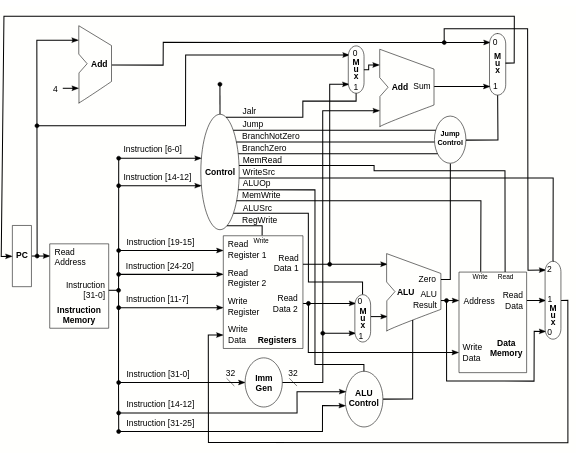
\includegraphics[scale=0.67]{riscv_ac2.png}
	\caption{RISC-V Graphic DataPath}
\end{figure}

\section{Parte B - Soma de Elementos de um Vetor}
\inputminted{asm}{./code/sumV.s}

\subsection{Organização em Memória}
\begin{table}[h]
    \centering
    \begin{tabular}{|c|c|}
        \hline
        \textbf{Endereço} & \textbf{Conteúdo} \\ \hline\hline
        0x100 & 5 - Tamanho vetor \\ \hline
        0x104 & 5 - v[0] \\ \hline
        0x108 & 4 - v[1] \\ \hline
        0x10C & 3 - v[2] \\ \hline
        0x110 & 2 - v[3] \\ \hline
        0x114 & 1 - v[4] \\ \hline
        (reg) a0 & 0x104 - v[0] \\ \hline
        (reg) a1 & 5 - Tamanho vetor \\ \hline
    \end{tabular}
\end{table}

\subsection{Execução}
\begin{table}[h]
    \centering
    \begin{tabular}{|c|c|c|}
        \hline
        \textbf{Etapa} & \textbf{Instrução} & \textbf{Resultado} \\ \hline\hline
        Inicialização & \texttt{add t0,zero,zero} & Soma = 0 \\ \hline
        Inicialização & \texttt{add t1,zero,zero} & Índice = 0 \\ \hline
        Comparação & \texttt{bge t1,a1,sum\_end} & Verifica $i \geq 5$ \\ \hline
        Offset & \texttt{slli t2,t1,2} & $t2 = i \times 4$ \\ \hline
        Endereço & \texttt{add t2,a0,t2} & Endereço de $v[i]$ \\ \hline
        Leitura & \texttt{lw t3,0(t2)} & Lê elemento \\ \hline
        Acumulação & \texttt{add t0,t0,t3} & Atualiza soma \\ \hline
        Incremento & \texttt{addi t1,t1,1} & Incrementa $i$ \\ \hline
        Repetição & \texttt{j sum\_loop} & Retorna ao loop \\ \hline
        Finalização & \texttt{add a0,t0,zero} & $a0 = 15$ \\ \hline
    \end{tabular}
\end{table}

\clearpage\subsection{Conversão para Binário}
As pseudoinstruções \fbox{\texttt{li}} e \fbox{\texttt{j}} correspondem a \fbox{\texttt{addi}} e \fbox{\texttt{jal x0}}.
\begin{table}[h]
    \centering
    \begin{tabular}{|c|c|c|}
        \hline
        \textbf{PC} & \textbf{Instrução} & \textbf{Binário} \\ \hline\hline
        0 & \texttt{li s0,0x100} & 00010000 00000000 00000100 00010011 \\ \hline
        4 & \texttt{li t0,5} & 00000000 01010000 00000010 10010011 \\ \hline
        8 & \texttt{sw t0,0(s0)} & 00000000 01010100 00100000 00100011 \\ \hline
        12 & \texttt{li t0,5} & 00000000 01010000 00000010 10010011 \\ \hline
        16 & \texttt{sw t0,4(s0)} & 00000000 01010100 00100010 00100011 \\ \hline
        20 & \texttt{li t0,4} & 00000000 01000000 00000010 10010011 \\ \hline
        24 & \texttt{sw t0,8(s0)} & 00000000 01010100 00100100 00100011 \\ \hline
        28 & \texttt{li t0,3} & 00000000 00110000 00000010 10010011 \\ \hline
        32 & \texttt{sw t0,12(s0)} & 00000000 01010100 00100110 00100011 \\ \hline
        36 & \texttt{li t0,2} & 00000000 00100000 00000010 10010011 \\ \hline
        40 & \texttt{sw t0,16(s0)} & 00000000 01010100 00101000 00100011 \\ \hline
        44 & \texttt{li t0,1} & 00000000 00010000 00000010 10010011 \\ \hline
        48 & \texttt{sw t0,20(s0)} & 00000000 01010100 00101010 00100011 \\ \hline
        52 & \texttt{addi a0,s0,4} & 00000000 01000100 00000101 00010011 \\ \hline
        56 & \texttt{lw a1,0(s0)} & 00000000 00000100 00100101 10000011 \\ \hline
        60 & \texttt{jal ra,sum\_vec} & 00000000 01000000 00000000 11101111 \\ \hline
        64 & \texttt{add t0,zero,zero} & 00000000 00000000 00000010 10110011 \\ \hline
        68 & \texttt{add t1,zero,zero} & 00000000 00000000 00000011 00110011 \\ \hline
        72 & \texttt{bge t1,a1,sum\_end} & 00000000 10110011 01011110 01100011 \\ \hline
        76 & \texttt{slli t2,t1,2} & 00000000 00100011 00010011 10010011 \\ \hline
        80 & \texttt{add t2,a0,t2} & 00000000 01110101 00000011 10110011 \\ \hline
        84 & \texttt{lw t3,0(t2)} & 00000000 00000011 10101110 00000011 \\ \hline
        88 & \texttt{add t0,t0,t3} & 00000001 11000010 10000010 10110011 \\ \hline
        92 & \texttt{addi t1,t1,1} & 00000000 00010011 00000011 00010011 \\ \hline
        96 & \texttt{j sum\_loop} & 11111110 10011111 11110000 01101111 \\ \hline
        100 & \texttt{add a0,t0,zero} & 00000000 00000010 10000101 00110011 \\ \hline
        104 & \texttt{j fim} & 00000000 01000000 00000000 01101111 \\ \hline
        108 & \texttt{j fim} & 00000000 00000000 00000000 01101111 \\ \hline
    \end{tabular}
\end{table}

\clearpage\subsection{Localização dos Bits - Barramento de Instrução}
\begin{table}[h]
    \centering
    \begin{tabular}{|c|c|c|}
        \hline
        \textbf{Bits} & \textbf{Campo} & \textbf{Destino na imagem} \\ \hline\hline
        6--0 & opcode & Control \\ \hline
        11--7 & rd & Registers -- Write Register \\ \hline
        14--12 & funct3 & Control e ALU Control \\ \hline
        19--15 & rs1 & Registers -- Read Register 1 \\ \hline
        24--20 & rs2 & Registers -- Read Register 2 \\ \hline
        31--25 & funct7, quando aplicável & ALU Control \\ \hline
        31--0 & Instrução completa & Imm Gen \\ \hline
    \end{tabular}
\end{table}

\subsection{Tipos de Instrução}
\begin{table}[h]
    \centering
    \begin{tabular}{|c|c|}
        \hline
        \textbf{Tipo} & \textbf{Instruções} \\ \hline\hline
        R & \texttt{add} \\ \hline
        I & \texttt{addi}, \texttt{li}, \texttt{lw}, \texttt{slli} \\ \hline
        S & \texttt{sw} \\ \hline
        B & \texttt{bge} \\ \hline
        J & \texttt{jal}, \texttt{j} \\ \hline
    \end{tabular}
\end{table}

\begin{center}
    \small
    \newlength{\largurabit}
    \setlength{\largurabit}{\dimexpr\linewidth/32-0.5pt\relax}

    R:
    \begin{bytefield}[endianness=big,bitwidth=\largurabit,bitheight=9mm]{32}
        \bitheader{31,25,24,20,19,15,14,12,11,7,6,0}\\
        \bitbox{7}[bgcolor=blue!20]{
            \shortstack{funct7}
        } &
        \bitbox{5}[bgcolor=green!20]{
            \shortstack{rs2}
        } &
        \bitbox{5}[bgcolor=yellow!25]{
            \shortstack{rs1}
        } &
        \bitbox{3}[bgcolor=red!20]{
            \shortstack{funct3}
        } &
        \bitbox{5}[bgcolor=cyan!20]{
            \shortstack{rd}
        } &
        \bitbox{7}[bgcolor=orange!20]{
            \shortstack{opcode}
        }
    \end{bytefield}

    \par\vspace{3mm}
    
    \small
    \newlength{\largurabitI}
    \setlength{\largurabitI}{\dimexpr\linewidth/32-0.5pt\relax}

    I:
    \begin{bytefield}[endianness=big,bitwidth=\largurabitI,bitheight=9mm]{32}
        \bitheader{31,20,19,15,14,12,11,7,6,0}\\
        \bitbox{12}[bgcolor=blue!20]{
            \shortstack{imm[11:0]}
        } &
        \bitbox{5}[bgcolor=yellow!20]{
            \shortstack{rs1}
        } &
        \bitbox{3}[bgcolor=red!20]{
            \shortstack{funct3}
        } &
        \bitbox{5}[bgcolor=cyan!20]{
            \shortstack{rd}
        } &
        \bitbox{7}[bgcolor=orange!20]{
            \shortstack{opcode}
        }
    \end{bytefield}

    \par\vspace{3mm}

    \small
    \newlength{\largurabitS}
    \setlength{\largurabitS}{\dimexpr\linewidth/32-0.5pt\relax}

    S:
    \begin{bytefield}[endianness=big,bitwidth=\largurabitS,bitheight=9mm]{32}
        \bitheader{31,25,24,20,19,15,14,12,11,7,6,0}\\
        \bitbox{7}[bgcolor=blue!20]{
            \shortstack{imm[11:5]}
        } &
        \bitbox{5}[bgcolor=green!20]{
            \shortstack{rs2}
        } &
        \bitbox{5}[bgcolor=yellow!25]{
            \shortstack{rs1}
        } &
        \bitbox{3}[bgcolor=red!20]{
            \shortstack{funct3}
        } &
        \bitbox{5}[bgcolor=cyan!20]{
            \shortstack{imm[4:0]}
        } &
        \bitbox{7}[bgcolor=orange!20]{
            \shortstack{opcode}
        }
    \end{bytefield}

    \par\vspace{3mm}
    
    \small
    \newlength{\largurabitB}
    \setlength{\largurabitB}{\dimexpr\linewidth/32-0.5pt\relax}

    B:
    \begin{bytefield}[endianness=big,bitwidth=\largurabitB,bitheight=9mm]{32}
        \bitheader{31,25,24,20,19,15,14,12,11,7,6,0}\\
        \bitbox{7}[bgcolor=blue!20]{
            \shortstack{\scriptsize imm[12|10:5]}
        } &
        \bitbox{5}[bgcolor=green!20]{
            \shortstack{rs2}
        } &
        \bitbox{5}[bgcolor=yellow!25]{
            \shortstack{rs1}
        } &
        \bitbox{3}[bgcolor=red!20]{
            \shortstack{funct3}
        } &
        \bitbox{5}[bgcolor=cyan!20]{
            \shortstack{\scriptsize imm[4:1|11]}
        } &
        \bitbox{7}[bgcolor=orange!20]{
            \shortstack{opcode}
        }
    \end{bytefield}

    \par\vspace{3mm}
    
    \small
    \newlength{\largurabitJ}
    \setlength{\largurabitJ}{\dimexpr\linewidth/32-0.5pt\relax}

    J:
    \begin{bytefield}[endianness=big,bitwidth=\largurabitJ,bitheight=9mm]{32}
        \bitheader{31,12,11,7,6,0}\\
        \bitbox{20}[bgcolor=blue!20]{
            \shortstack{imm[20|10:1|11|19:12]}
        } &
        \bitbox{5}[bgcolor=cyan!20]{
            \shortstack{rd}
        } &
        \bitbox{7}[bgcolor=orange!20]{
            \shortstack{opcode}
        }
    \end{bytefield}
\end{center}


\clearpage\subsection{Análise do Datapath por Instrução}
\begin{table}[h]
    \small
    \centering
    \begin{tabular}{|c|c|c|c|}
        \hline
        \multicolumn{4}{|c|}{\textbf{Datapath - Blocos Comuns}} \\ \hline\hline
        PC & Instruction Memory & Control & Somador \textit{(PC+4)} \\ \hline
    \end{tabular}
\end{table}

\subsubsection{Inicialização e Acesso à Memória}
\begin{table}[h]
    \small
    \centering
    \begin{tabularx}{\linewidth}{|c|X|X|}
        \hline
        \textbf{Instrução} & \textbf{Datapath} & \textbf{Operação} \\ \hline\hline
        \texttt{li} & Registradores, Imm Gen, ALU Control, ALU e multiplexadores & Carrega uma constante \\ \hline
        \texttt{addi} & Registradores, Imm Gen, ALU Control, ALU e multiplexadores & Soma registrador e imediato \\ \hline
        \texttt{sw} & Registradores, Imm Gen, ALU Control, ALU e Data Memory & Escreve na memória \\ \hline
        \texttt{lw} & Registradores, Imm Gen, ALU Control, ALU, Data Memory e multiplexadores & Lê da memória \\ \hline
    \end{tabularx}
\end{table}

\subsubsection{Operações Aritméticas e Deslocamento}
\begin{table}[h]
    \small
    \centering
    \begin{tabularx}{\linewidth}{|c|>{\raggedright\arraybackslash}X|>{\raggedright\arraybackslash}X|}
        \hline
        \textbf{Instrução} & \textbf{Datapath} & \textbf{Operação} \\ \hline\hline
        \texttt{add} & Registradores, ALU Control, Mux ALUSrc, ALU, Mux WriteSrc & Soma dois registradores \\ \hline
        \texttt{slli} & Registradores, Imm Gen, ALU Control, Mux ALUSrc, ALU, Mux WriteSrc & Desloca bits à esquerda \\ \hline
    \end{tabularx}
\end{table}

\clearpage\subsubsection{Desvios e Saltos}
\begin{table}[h]
    \small
    \centering
    \begin{tabularx}{\linewidth}{|c|>{\raggedright\arraybackslash}X|>{\raggedright\arraybackslash}X|}
        \hline
        \textbf{Instrução} & \textbf{Datapath} & \textbf{Operação} \\ \hline\hline
        \texttt{bge} & Registradores, Imm Gen, ALU Control, ALU, Jump Control, Add Sum, Mux PC & Desvia se maior ou igual \\ \hline
        \texttt{jal} & Registradores, Imm Gen, Add Sum, Jump Control, Mux PC, Mux WriteSrc & Salta e salva PC+4 \\ \hline
        \texttt{j} & Imm Gen, Add Sum, Jump Control, Mux PC & Salto incondicional \\ \hline
    \end{tabularx}
\end{table}

\clearpage\subsection{Sinais de Controle}
\subsubsection{Registradores e Memórias}
\begin{table}[h]
    \centering
    \small
    \begin{tabularx}{\linewidth}{|c|c|c|c|c|>{\centering\arraybackslash}X|}
        \hline
        \textbf{Instrução} & \textbf{RegWrite} & \textbf{MemRead} & \textbf{MemWrite} & \textbf{ALUSrc} & \textbf{WriteSrc} \\ \hline\hline
        \texttt{li}   & 1 & 0 & 0 & 1 & 00 \\ \hline
        \texttt{addi} & 1 & 0 & 0 & 1 & 00 \\ \hline
        \texttt{sw}   & 0 & 0 & 1 & 1 & -- \\ \hline
        \texttt{lw}   & 1 & 1 & 0 & 1 & 01 \\ \hline
        \texttt{add}  & 1 & 0 & 0 & 0 & 00 \\ \hline
        \texttt{slli} & 1 & 0 & 0 & 1 & 00 \\ \hline
        \texttt{bge}  & 0 & 0 & 0 & 0 & -- \\ \hline
        \texttt{jal}  & 1 & 0 & 0 & -- & 10 \\ \hline
        \texttt{j}    & 1 & 0 & 0 & -- & 10 \\ \hline
    \end{tabularx}
\end{table}

\subsubsection{ALU e desvios}
\begin{table}[h]
    \centering
    \small
    \begin{tabularx}{\linewidth}{|c|c|c|c|>{\centering\arraybackslash}X|>{\centering\arraybackslash}X|}
        \hline
        \textbf{Instrução} & \textbf{ALU} & \textbf{Jump} & \textbf{Jalr} & \textbf{BranchZero} & \textbf{BranchNotZero} \\ \hline\hline
        \texttt{li}   & ADD & 0 & 0 & 0 & 0 \\ \hline
        \texttt{addi} & ADD & 0 & 0 & 0 & 0 \\ \hline
        \texttt{sw}   & ADD & 0 & 0 & 0 & 0 \\ \hline
        \texttt{lw}   & ADD & 0 & 0 & 0 & 0 \\ \hline
        \texttt{add}  & ADD & 0 & 0 & 0 & 0 \\ \hline
        \texttt{slli} & SLL & 0 & 0 & 0 & 0 \\ \hline
        \texttt{bge}  & SLT & 0 & 0 & 1 & 0 \\ \hline
        \texttt{jal}  & --  & 1 & 0 & 0 & 0 \\ \hline
        \texttt{j}    & --  & 1 & 0 & 0 & 0 \\ \hline
    \end{tabularx}
\end{table}

\clearpage\subsection{Datapath - Representação Gráfica}
\subsubsection{Inicialização e Acesso à Memória}
\begin{figure}[h]
    \centering
    \caption*{Load Immediate}
    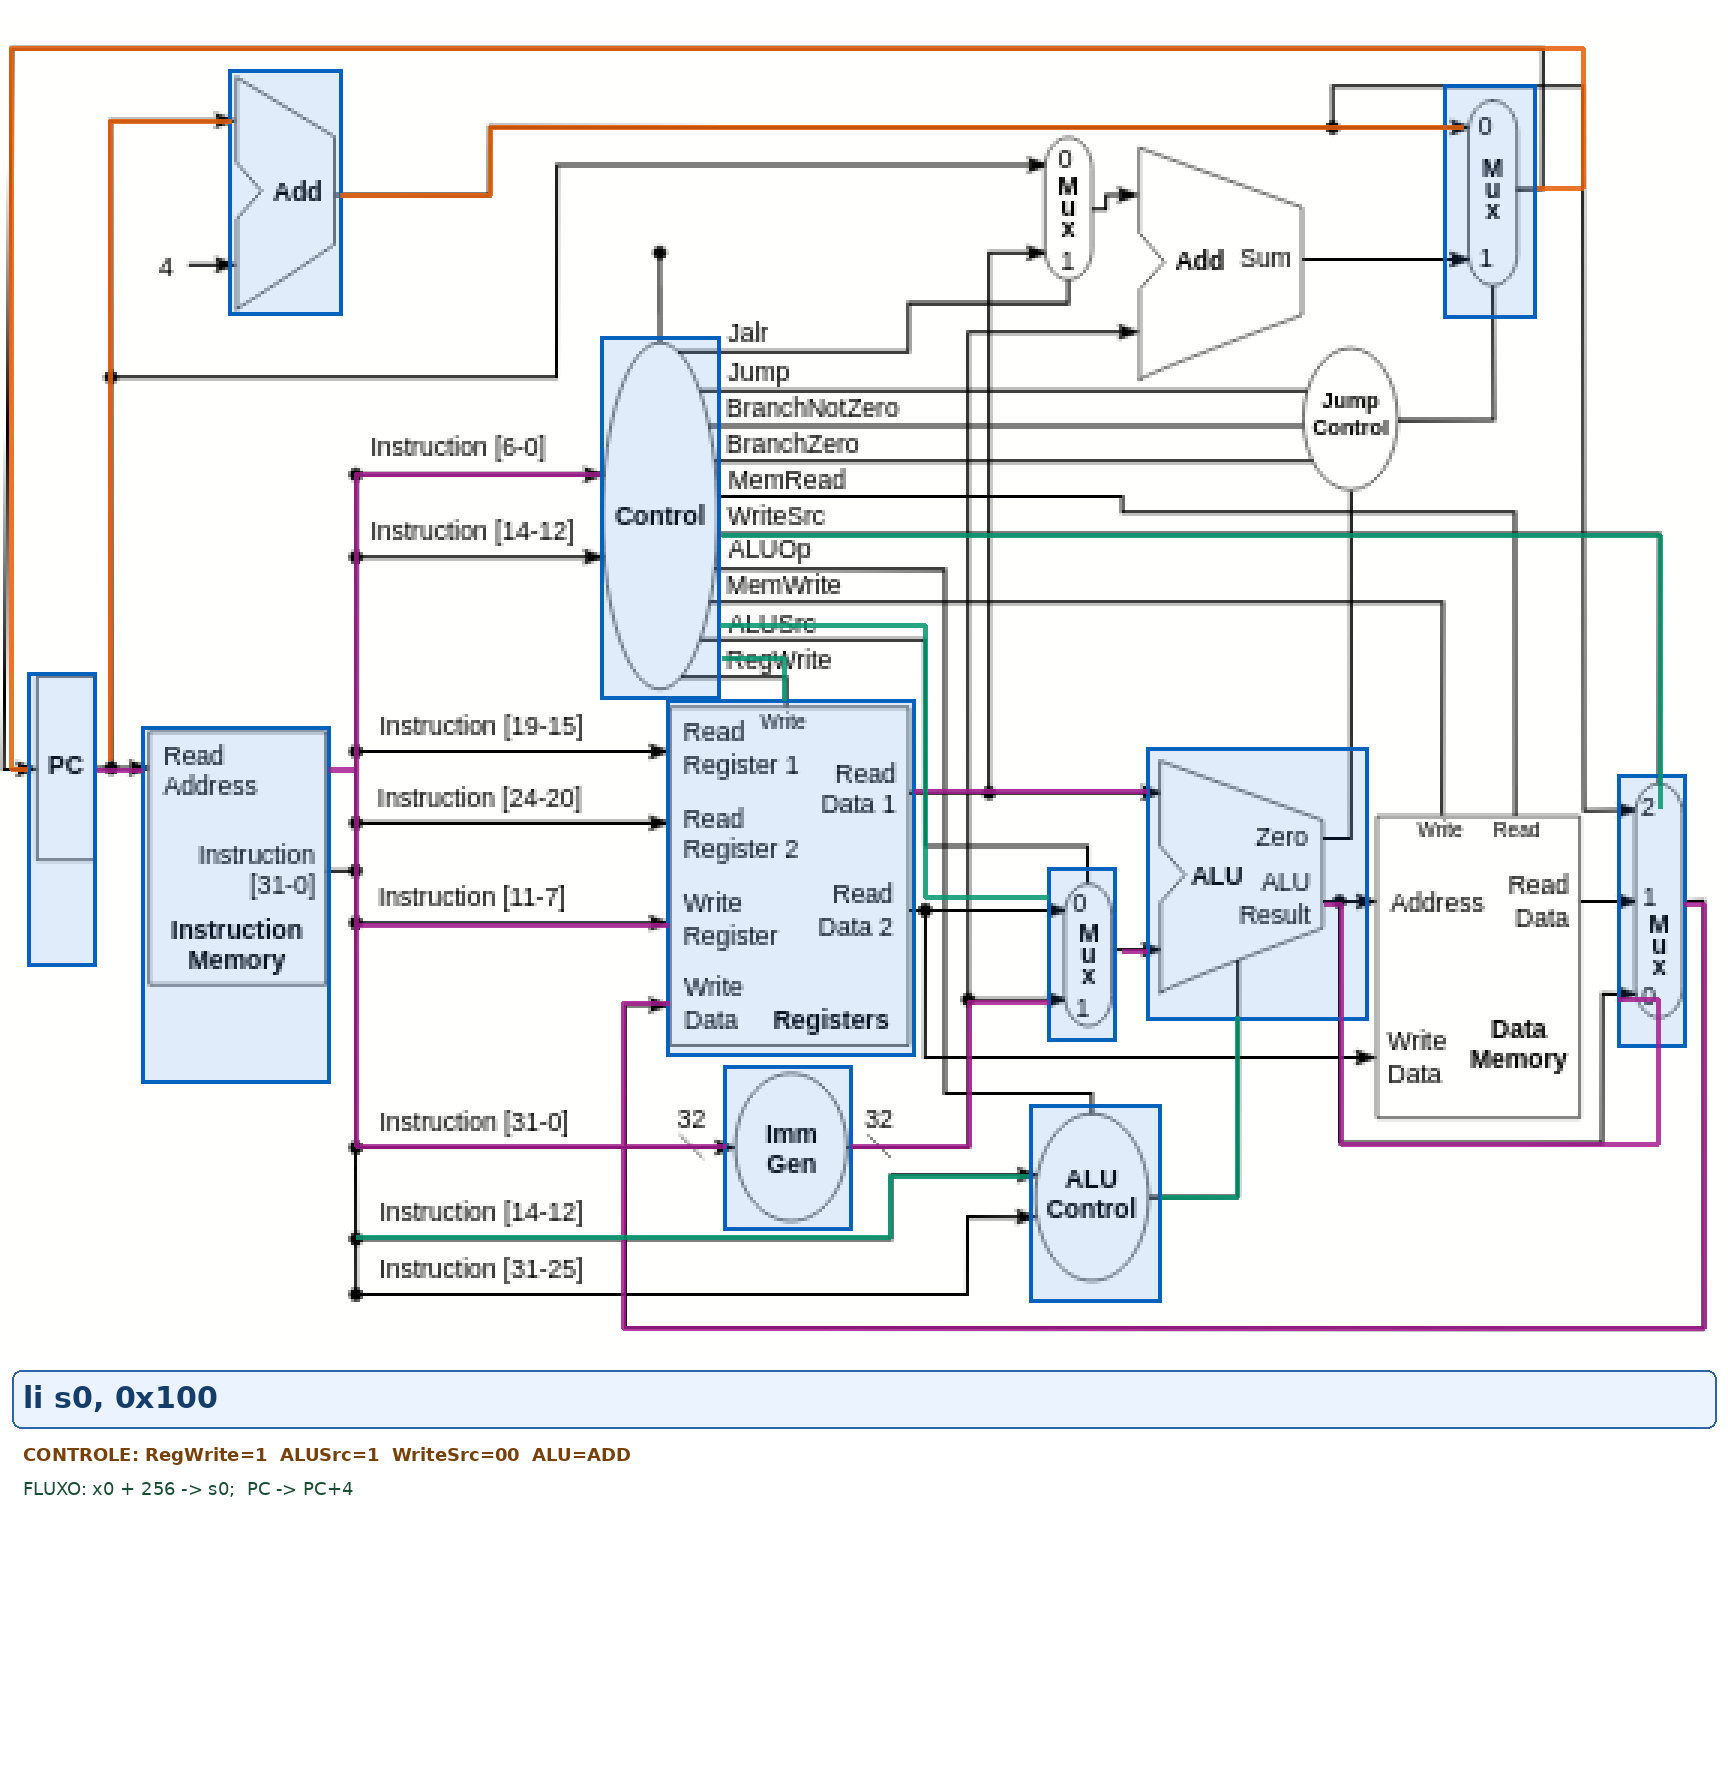
\includegraphics[scale=0.215]{./img/dp_mem/01_datapath.png}
\end{figure}

\clearpage\begin{figure}
    \centering
    \caption*{Add Immediate}
    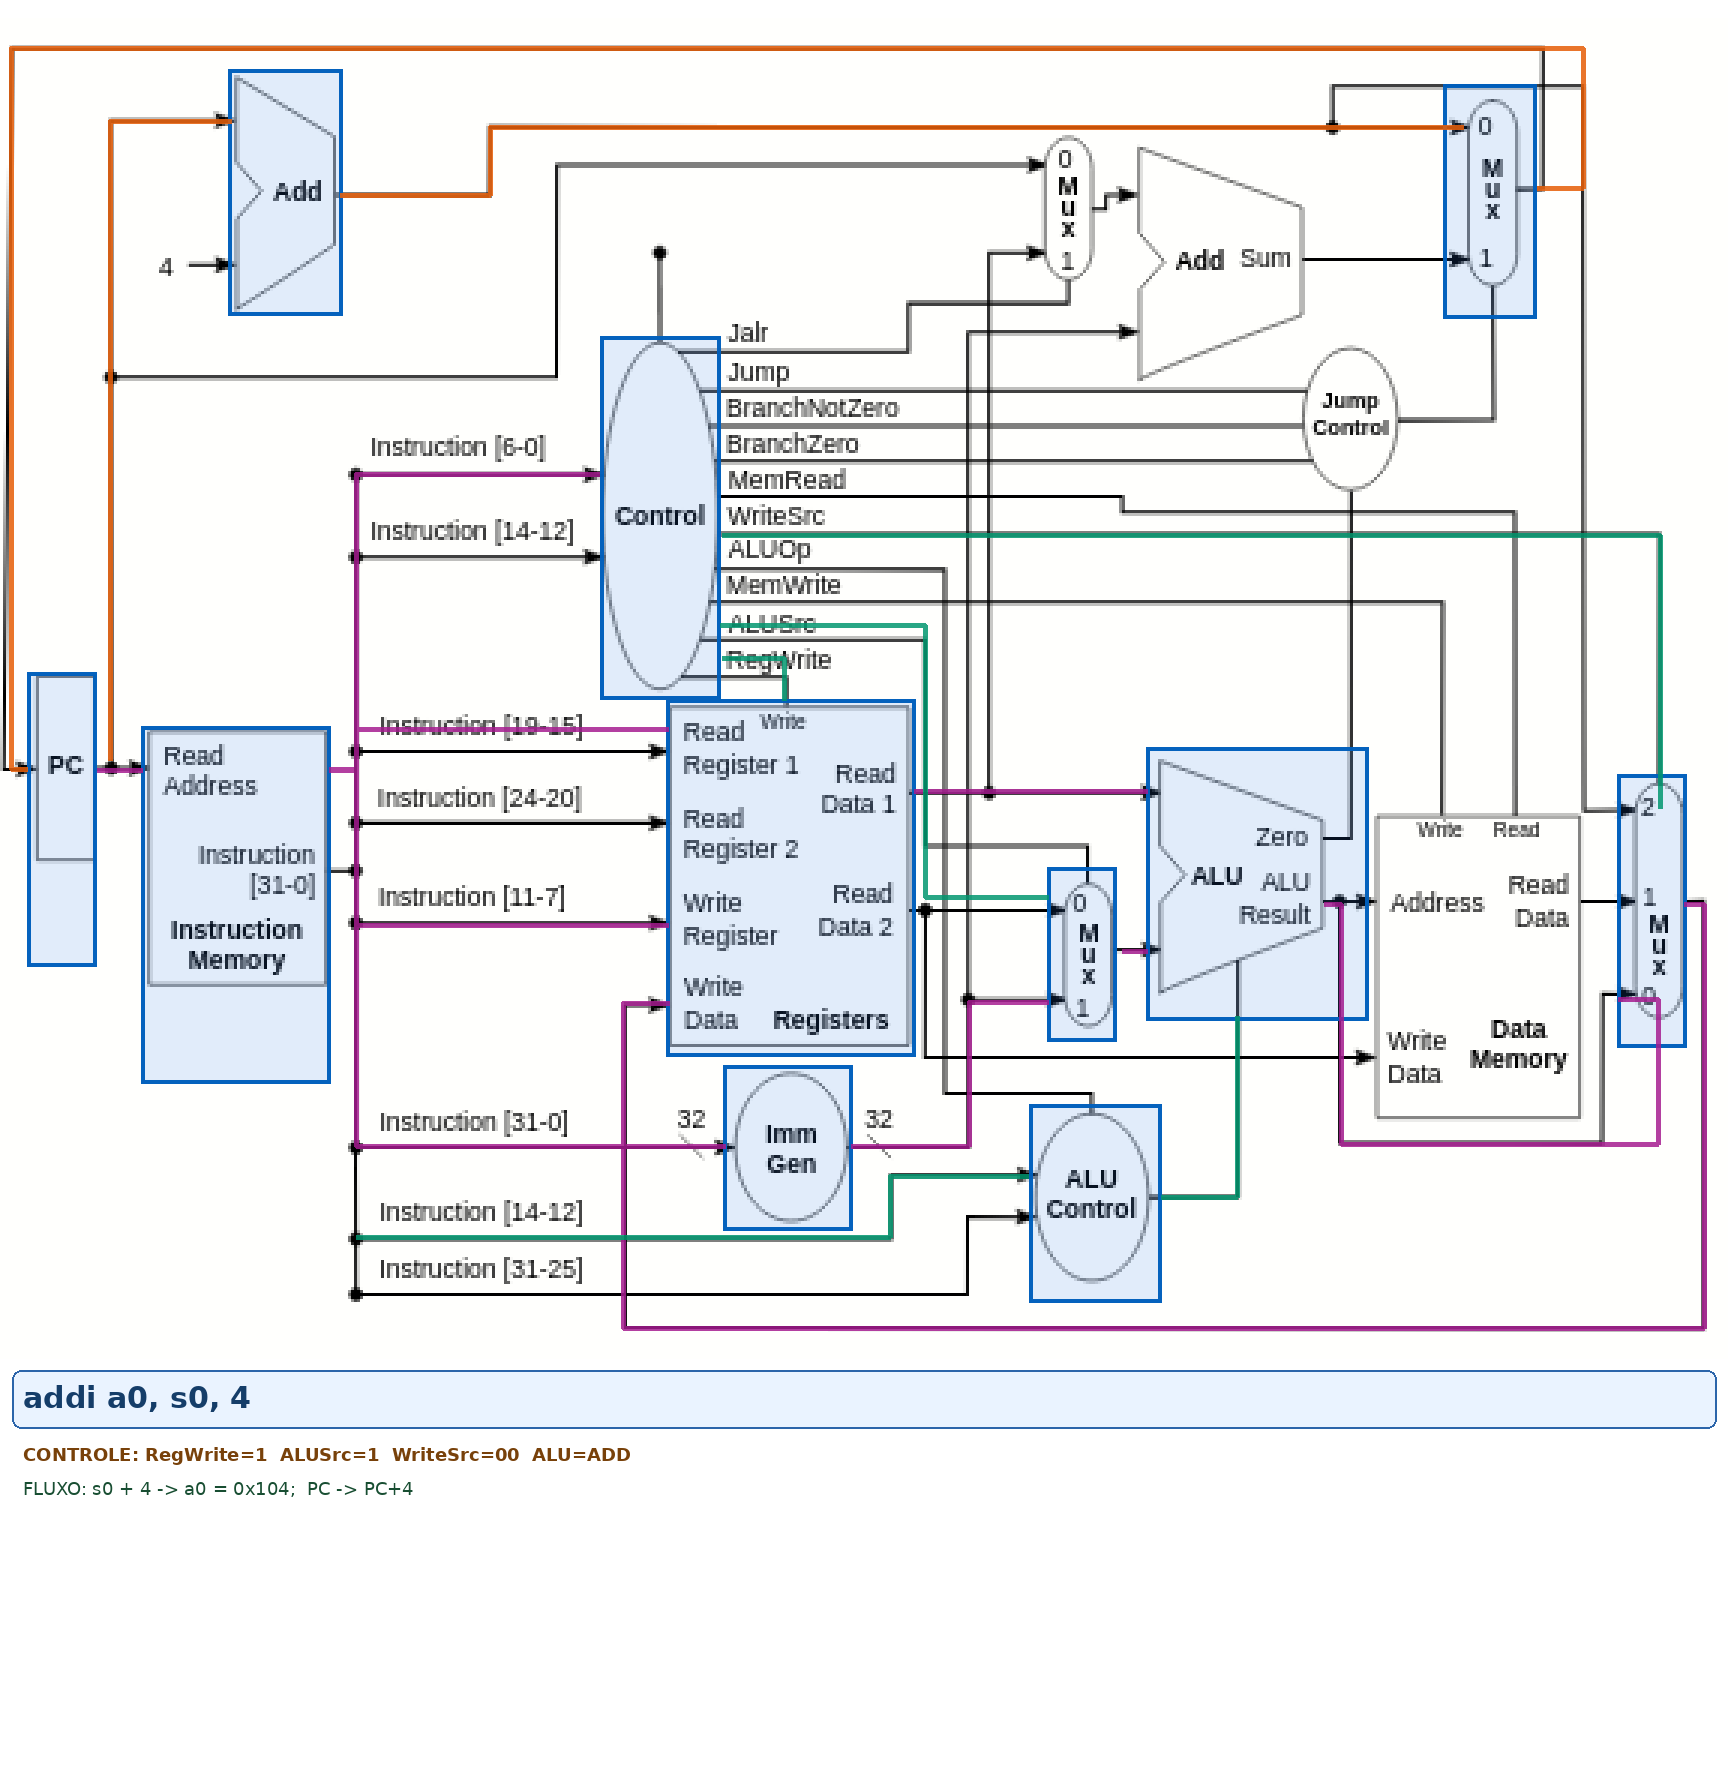
\includegraphics[width=\linewidth]{./img/dp_mem/02_datapath.png}
\end{figure}

\clearpage\begin{figure}
    \centering
    \caption*{Store Word}
    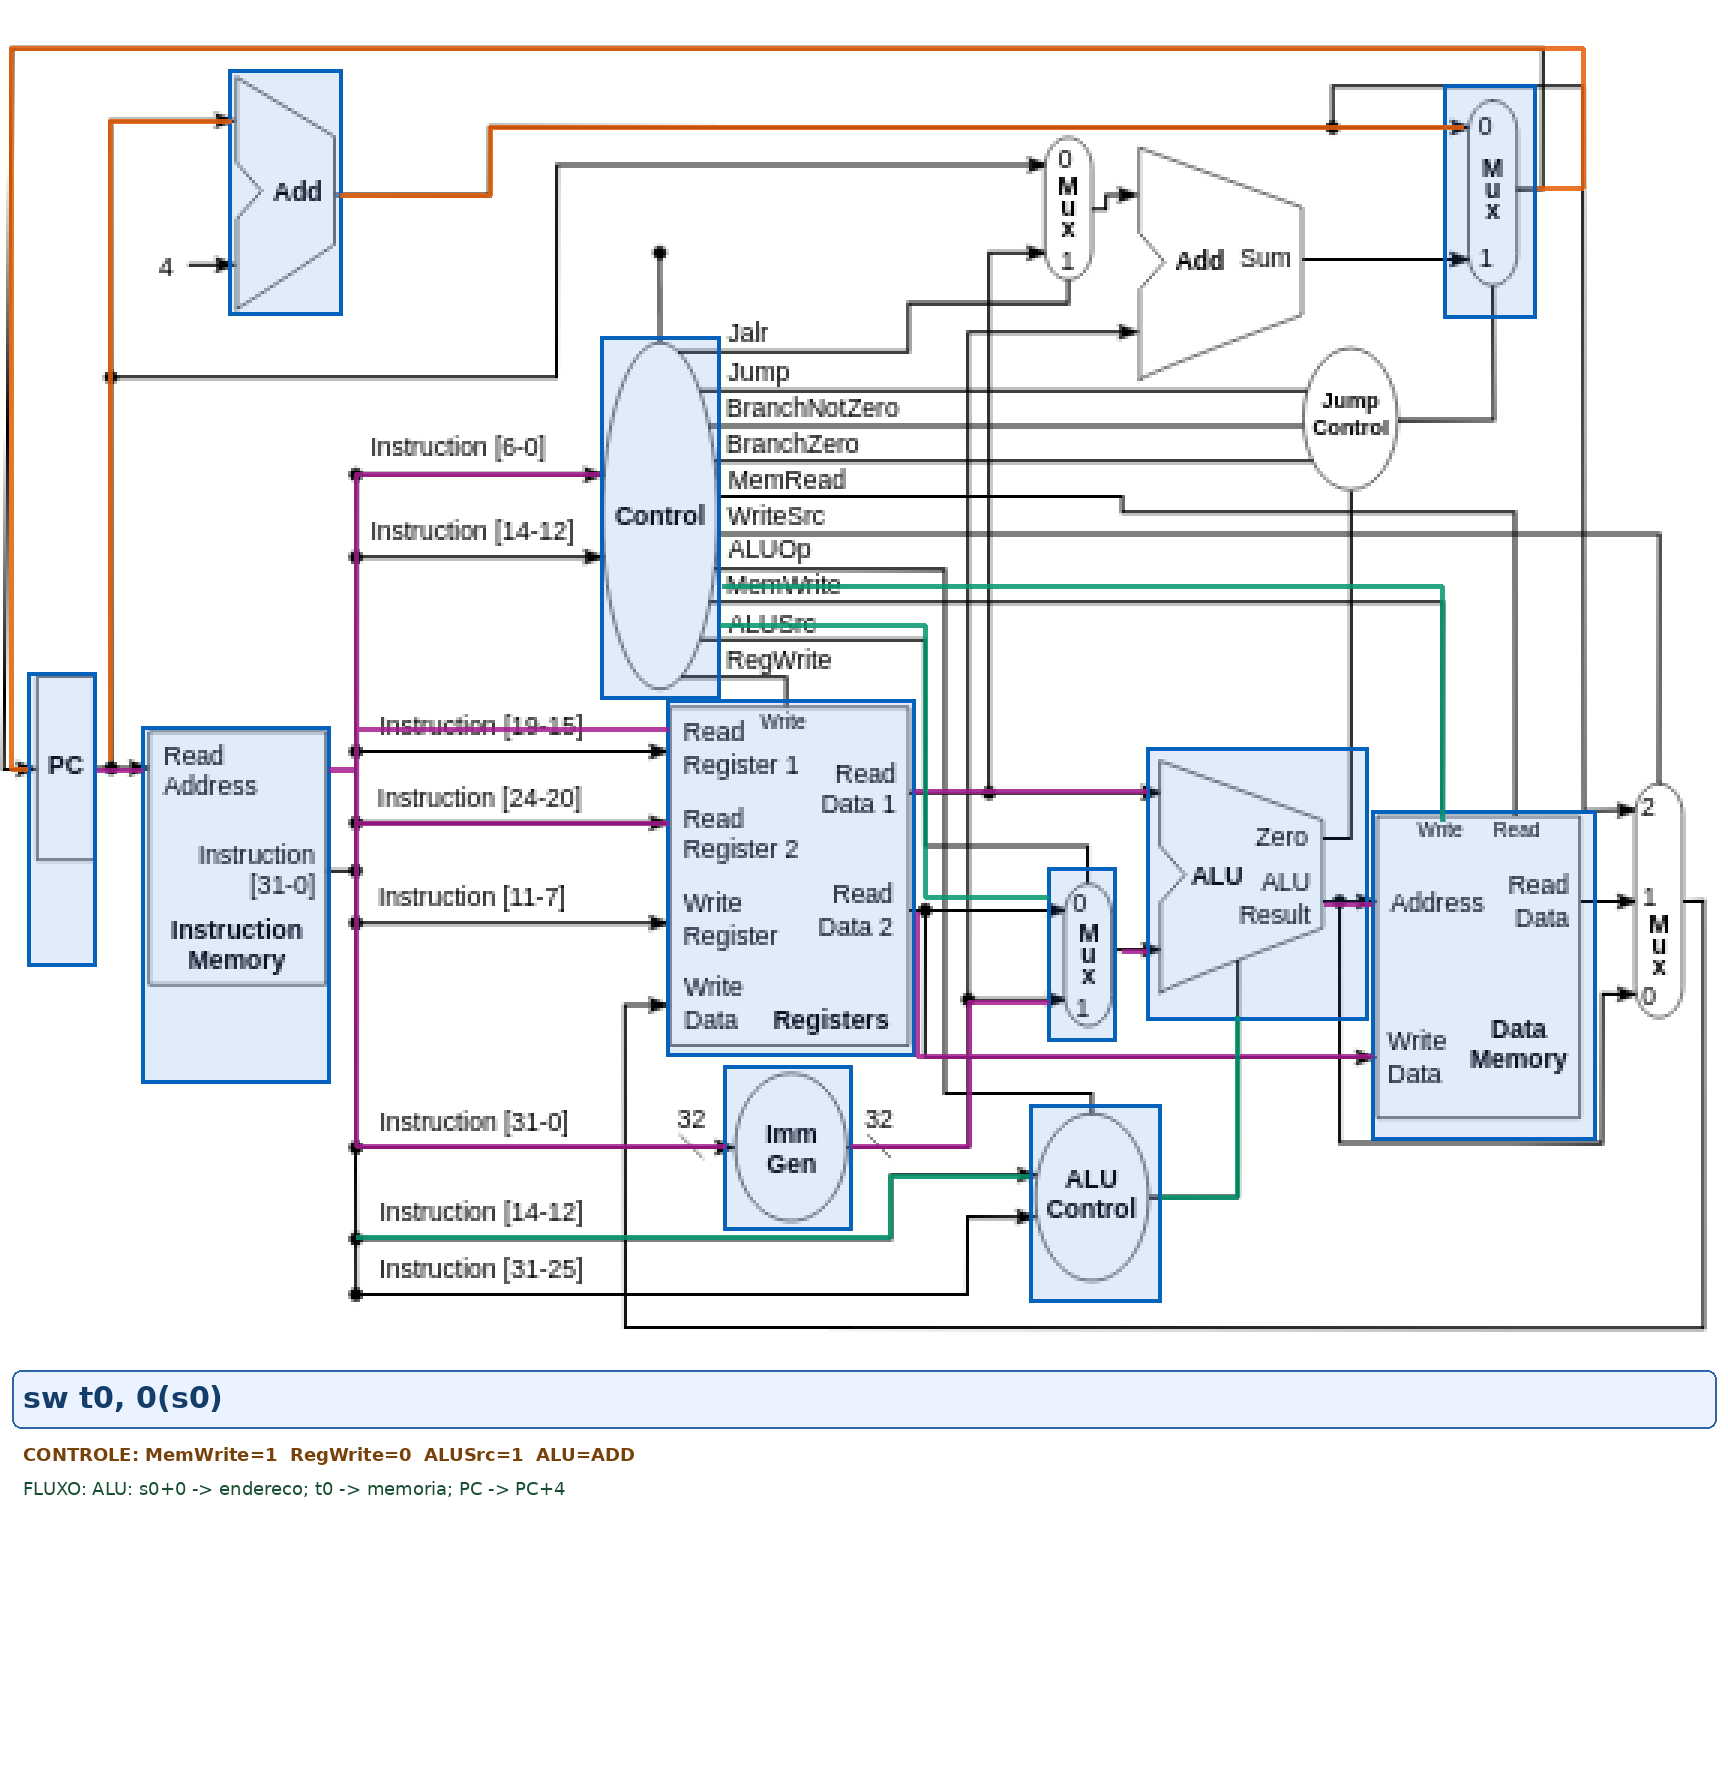
\includegraphics[width=\linewidth]{./img/dp_mem/03_datapath.png}
\end{figure}

\clearpage\begin{figure}
    \centering
    \caption*{Load Word}
    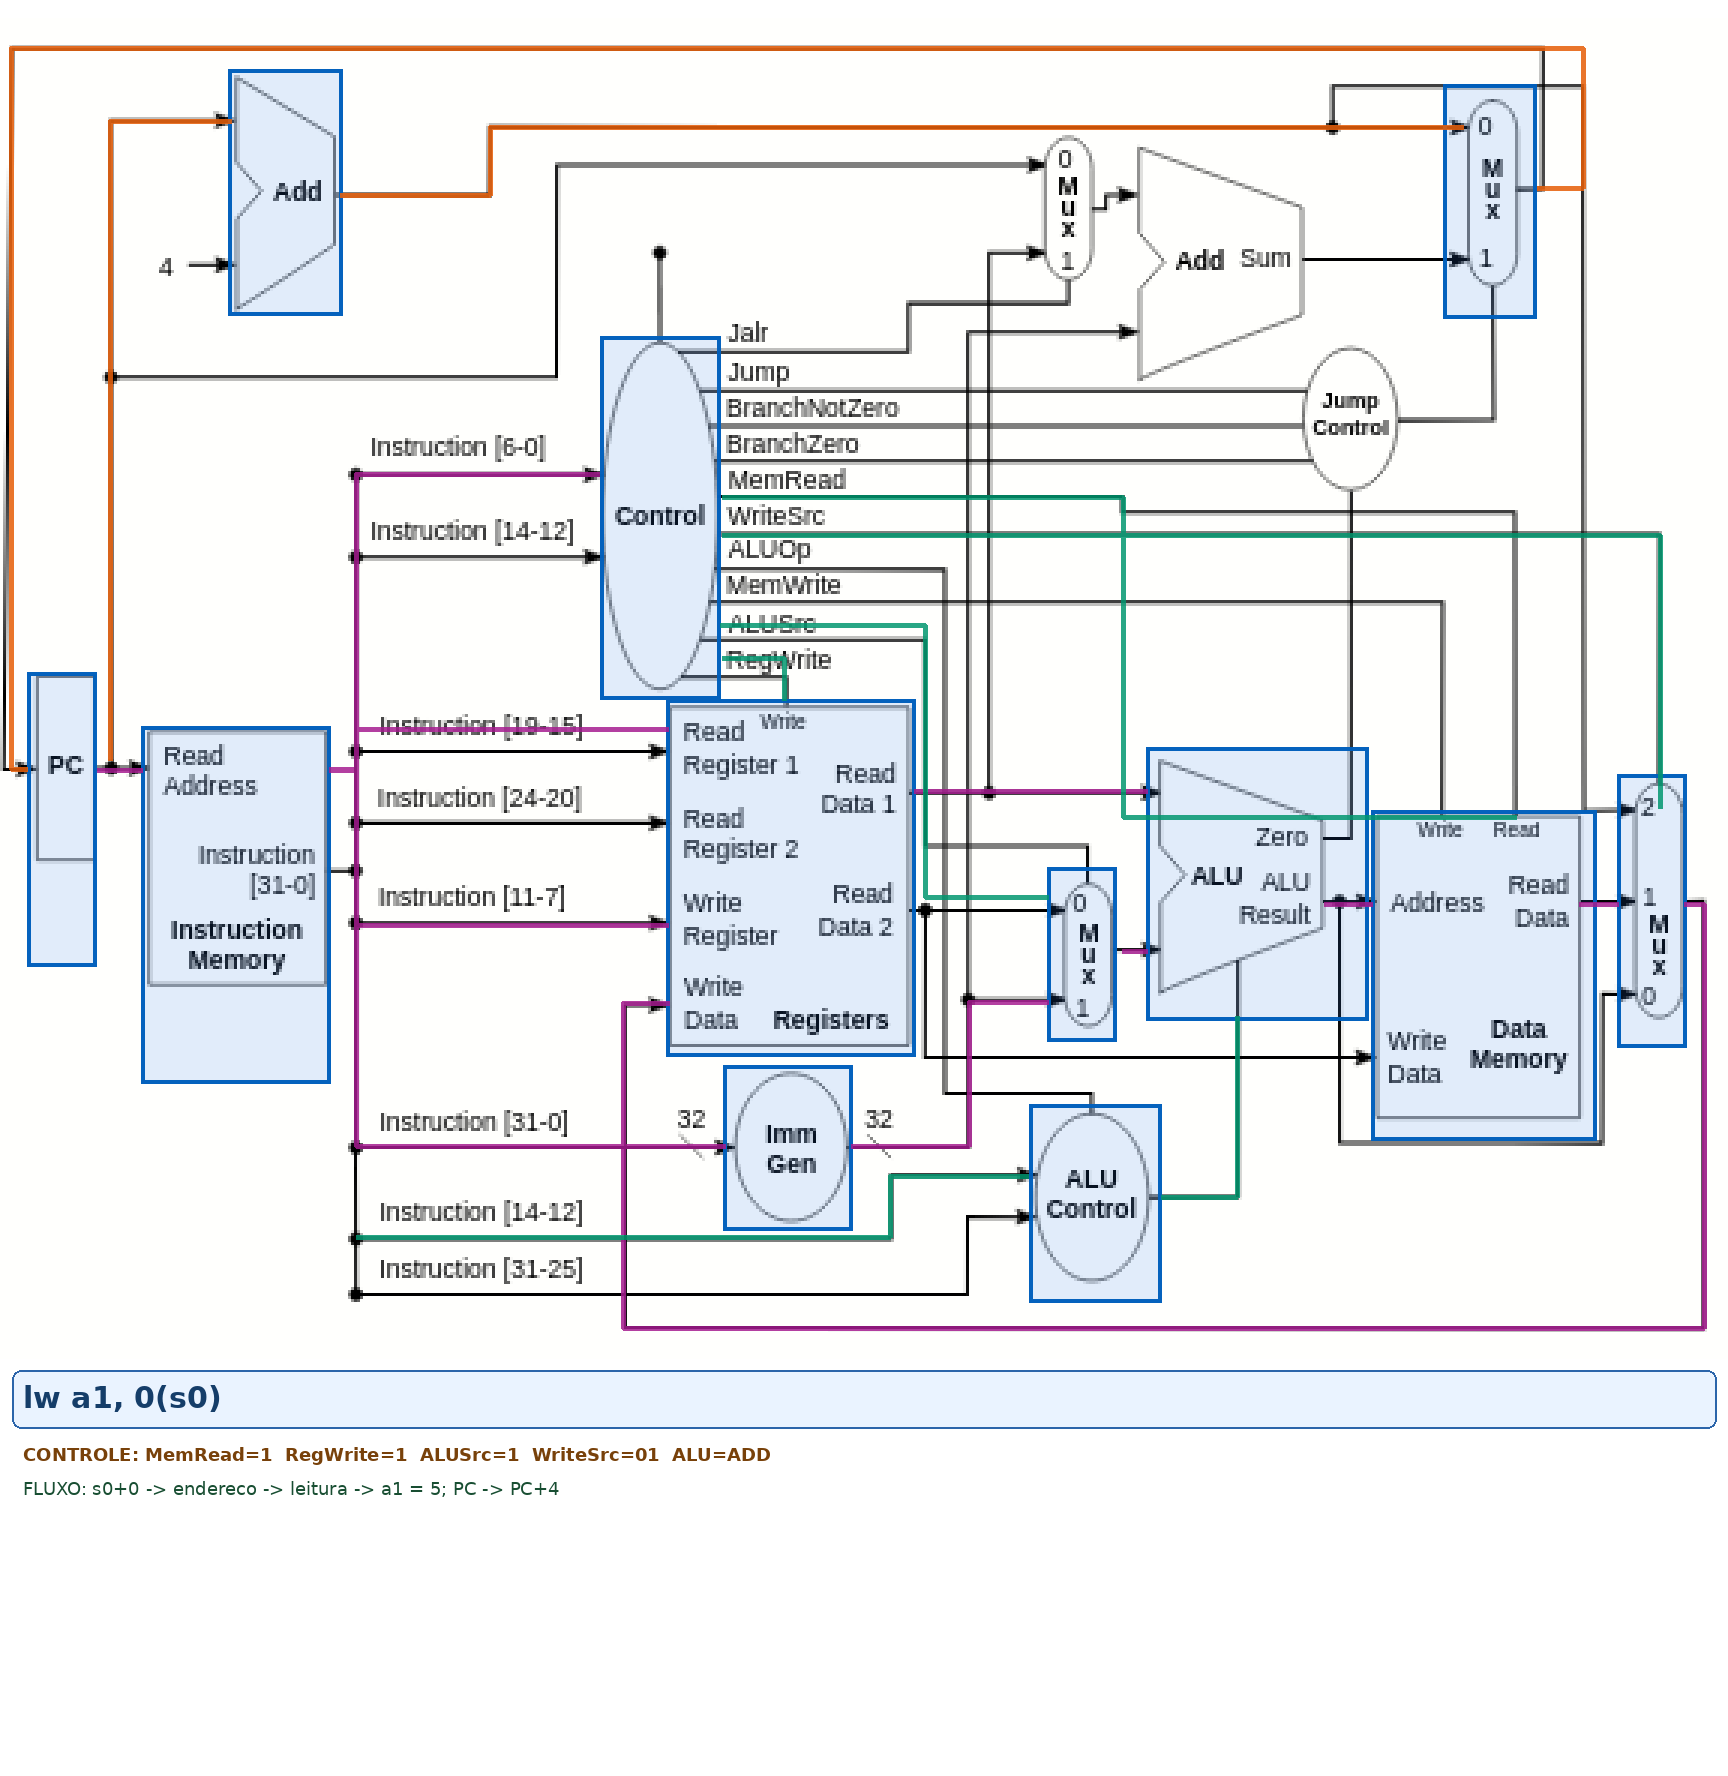
\includegraphics[width=\linewidth]{./img/dp_mem/04_datapath.png}
\end{figure}


\clearpage\subsubsection{Operações Aritméticas e Deslocamento}
\begin{figure}[h]
    \centering
    \caption*{Add}
    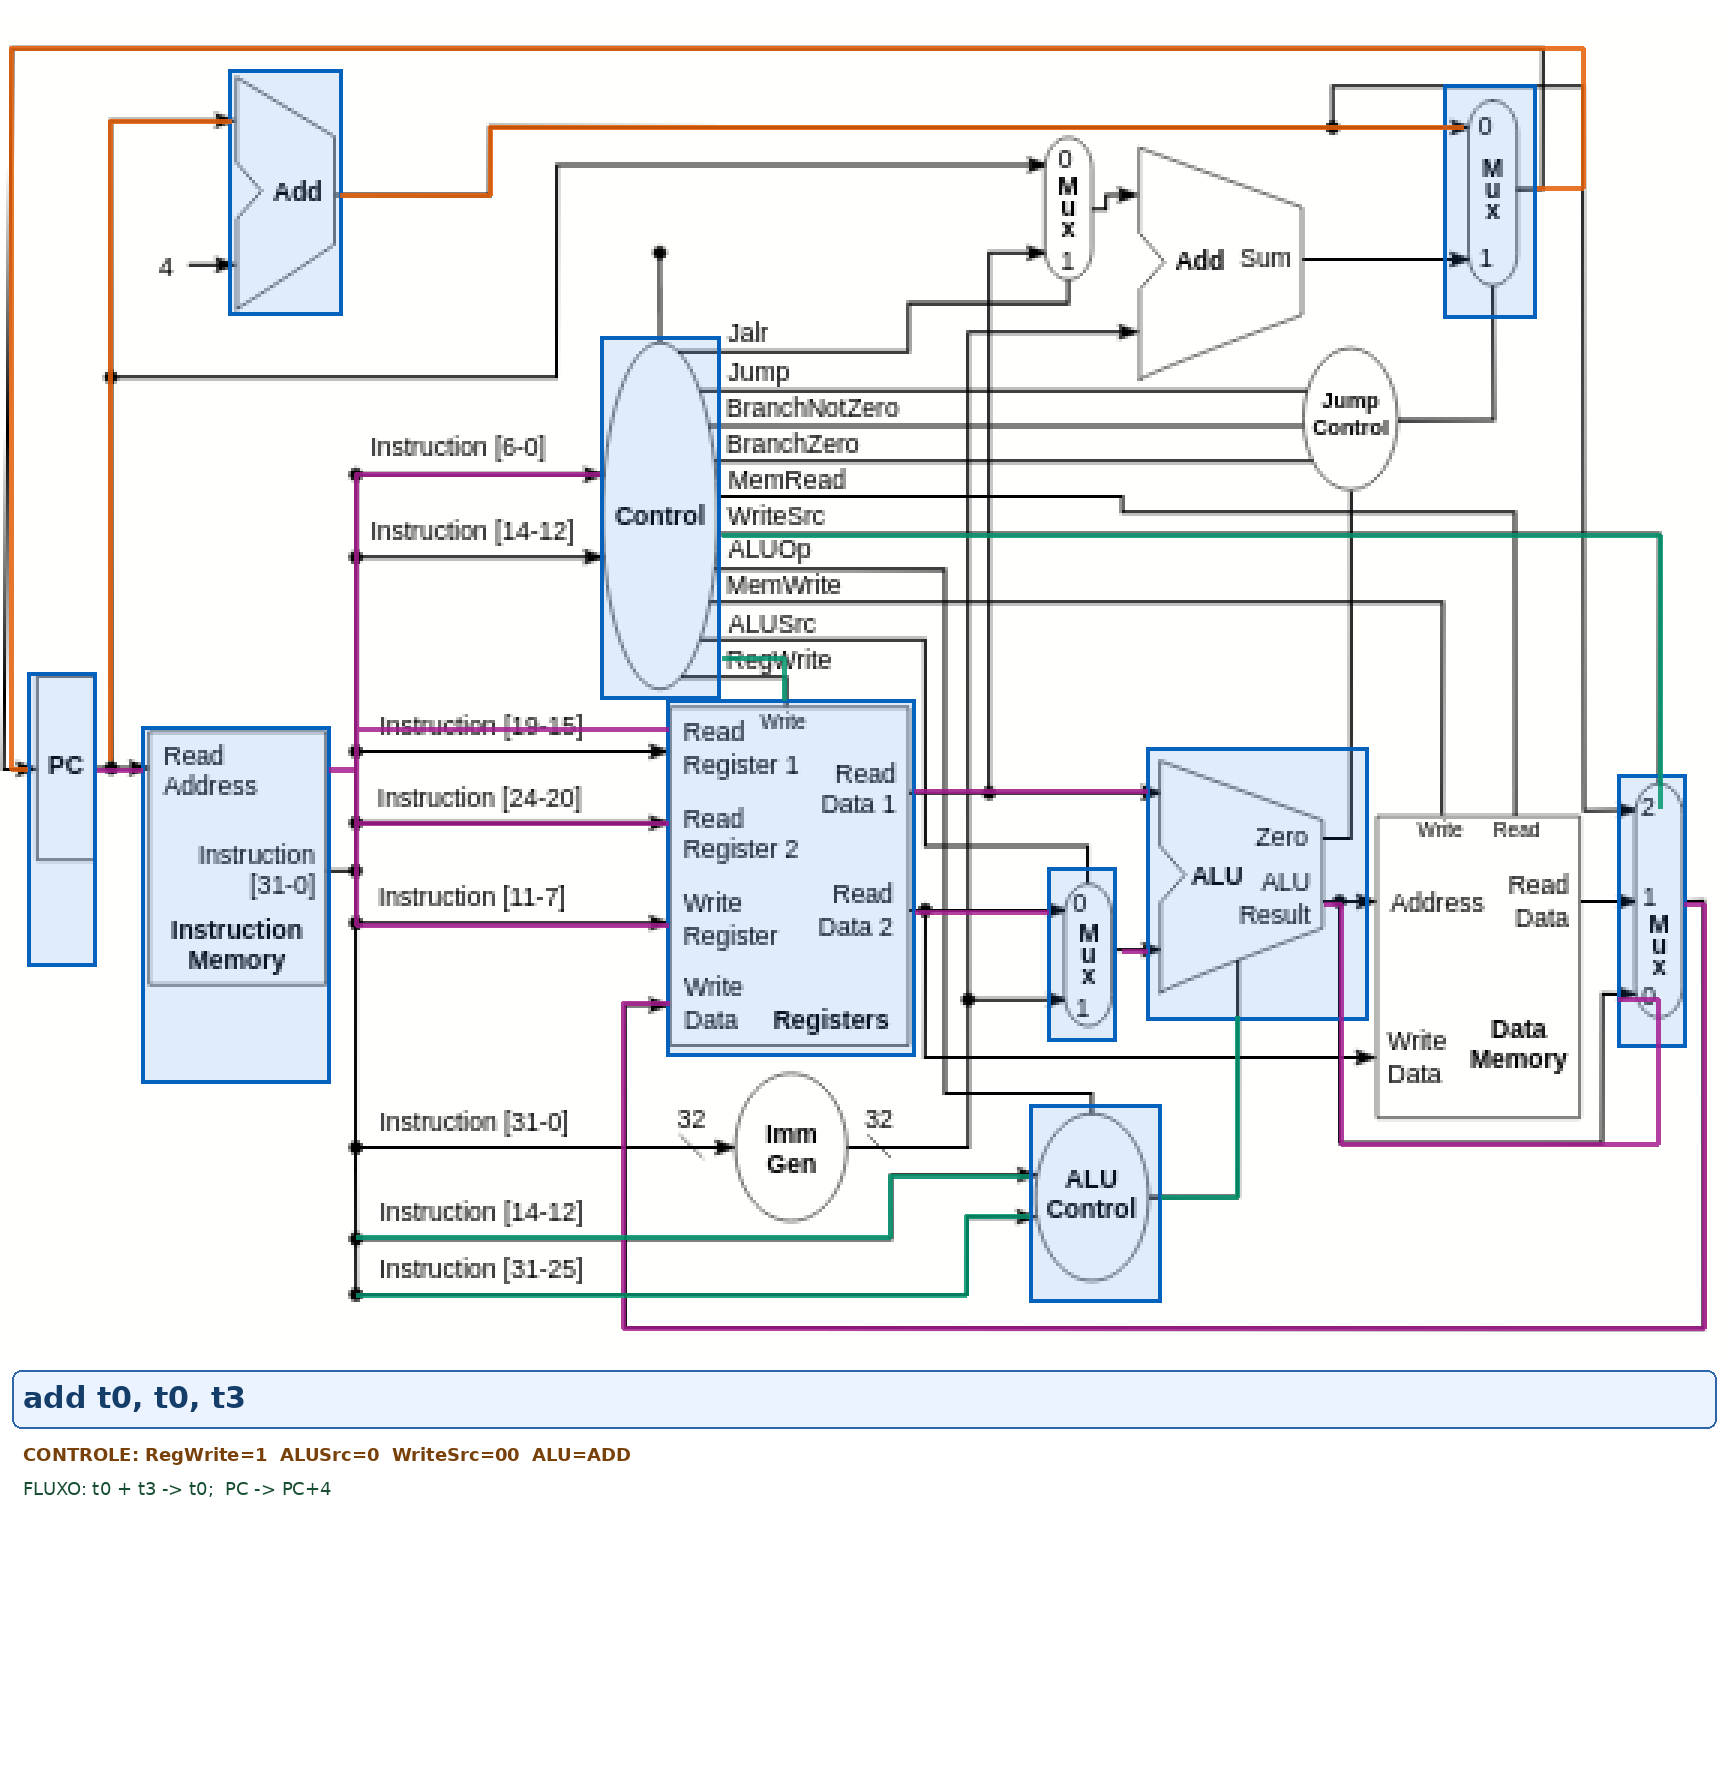
\includegraphics[scale=0.23]{./img/dp_op/05_datapath.png}
\end{figure}

\clearpage\begin{figure}
    \centering
    \caption*{Shift Left Logical Immediate}
    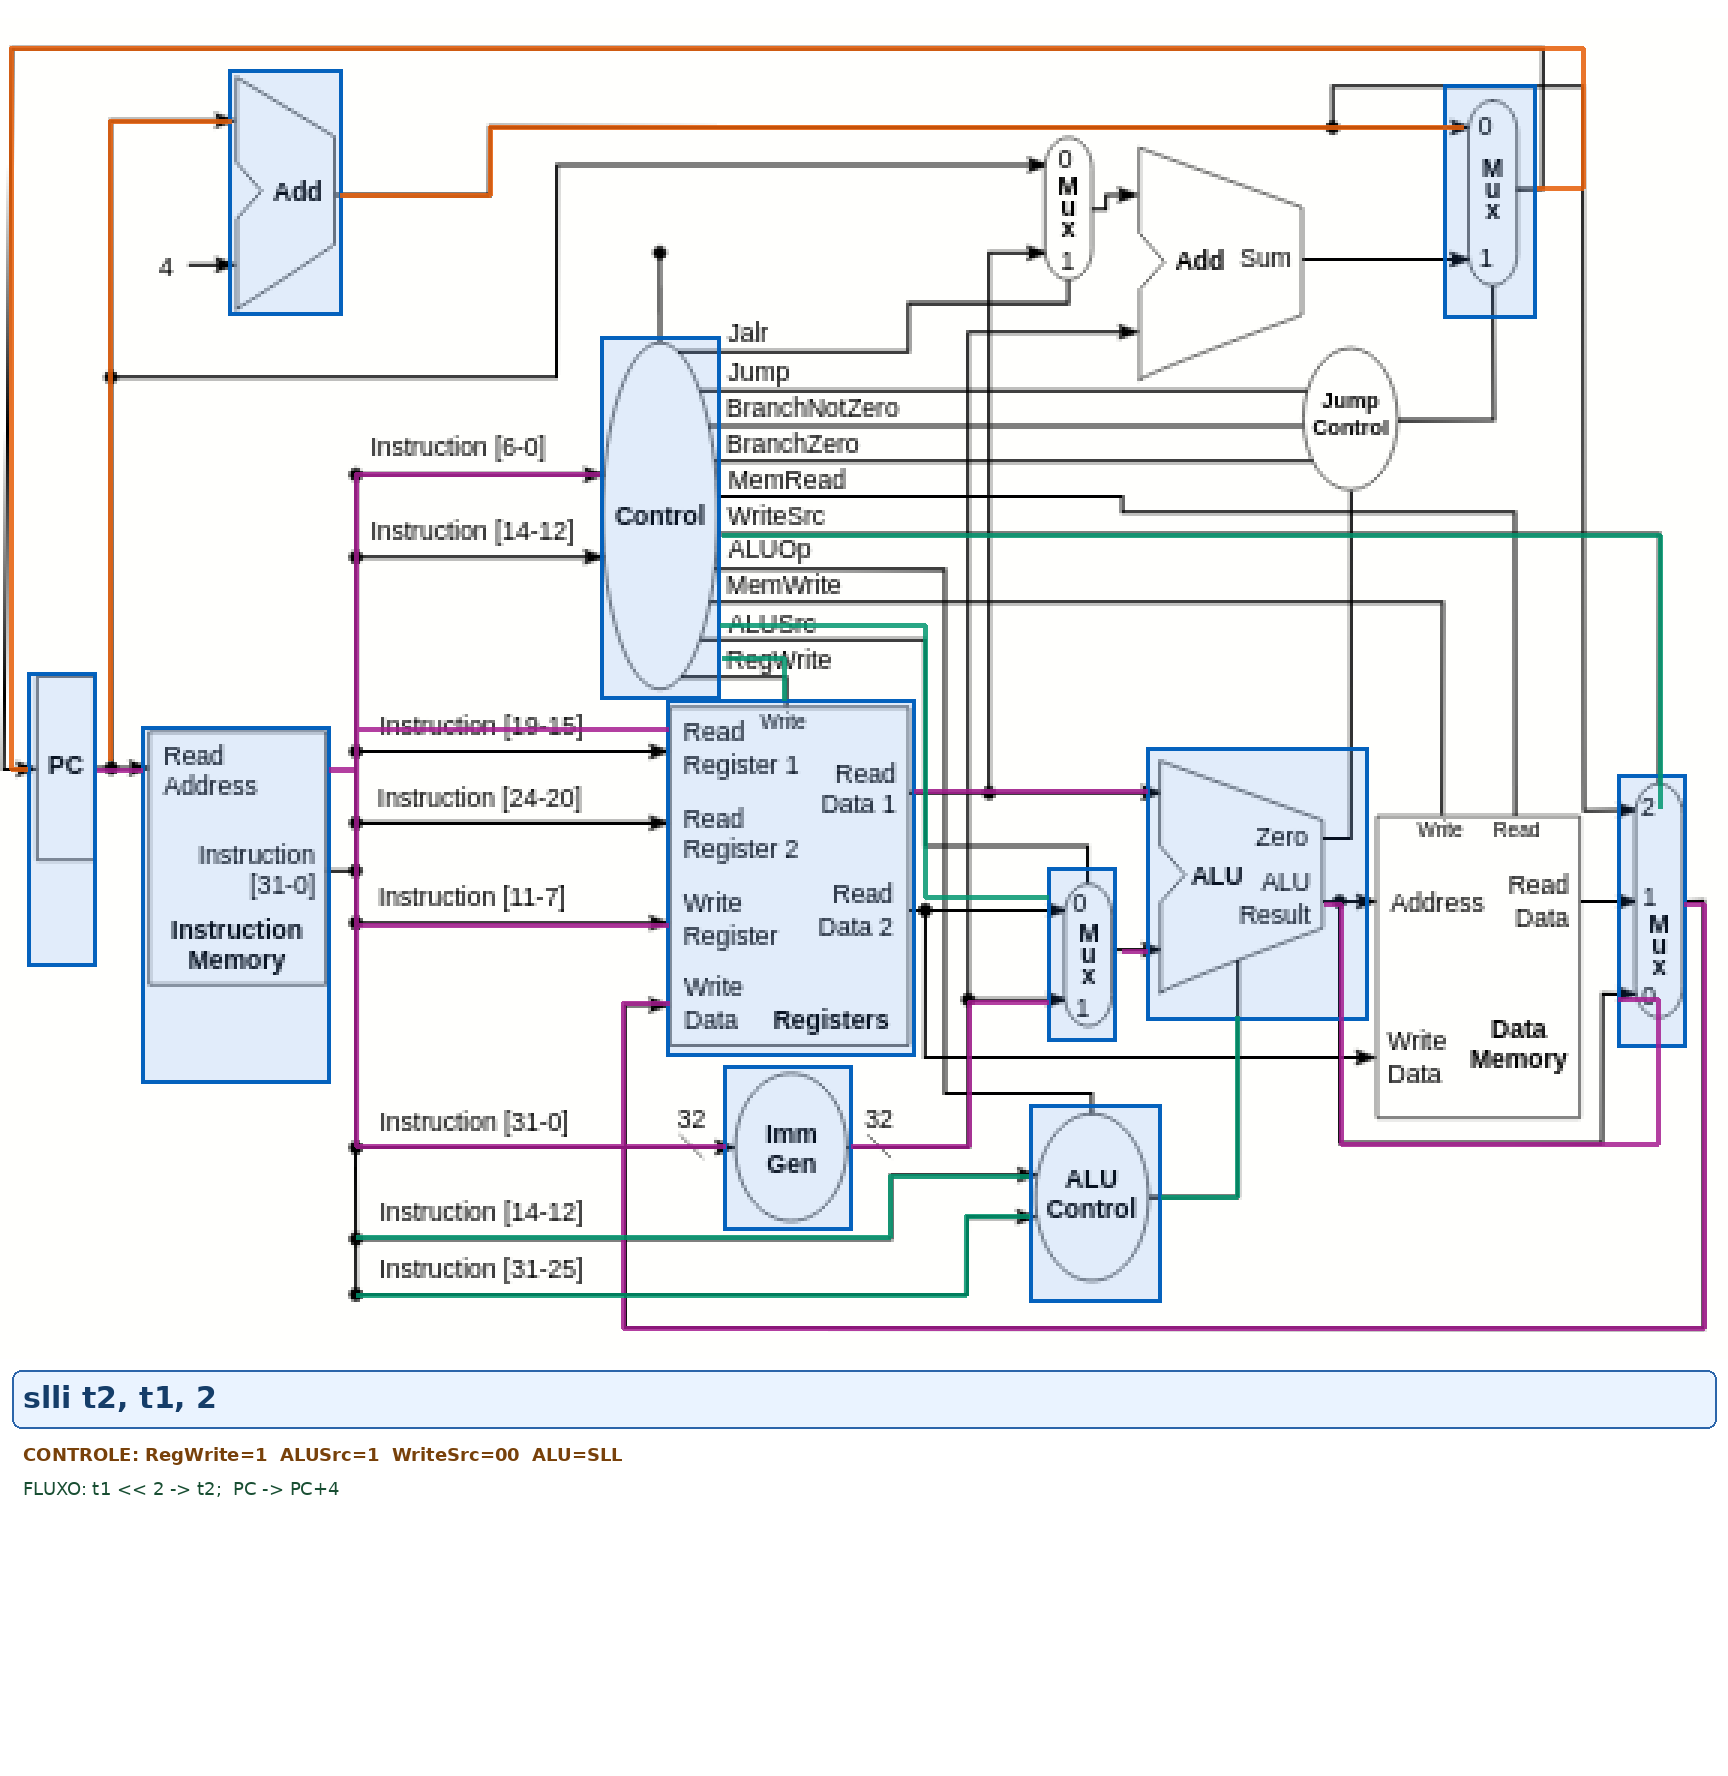
\includegraphics[width=\linewidth]{./img/dp_op/06_datapath.png}
\end{figure}



\clearpage\subsubsection{Desvios e Saltos}
\begin{figure}[h]
    \centering
    \caption*{Branch if Greater Than or Equal}
    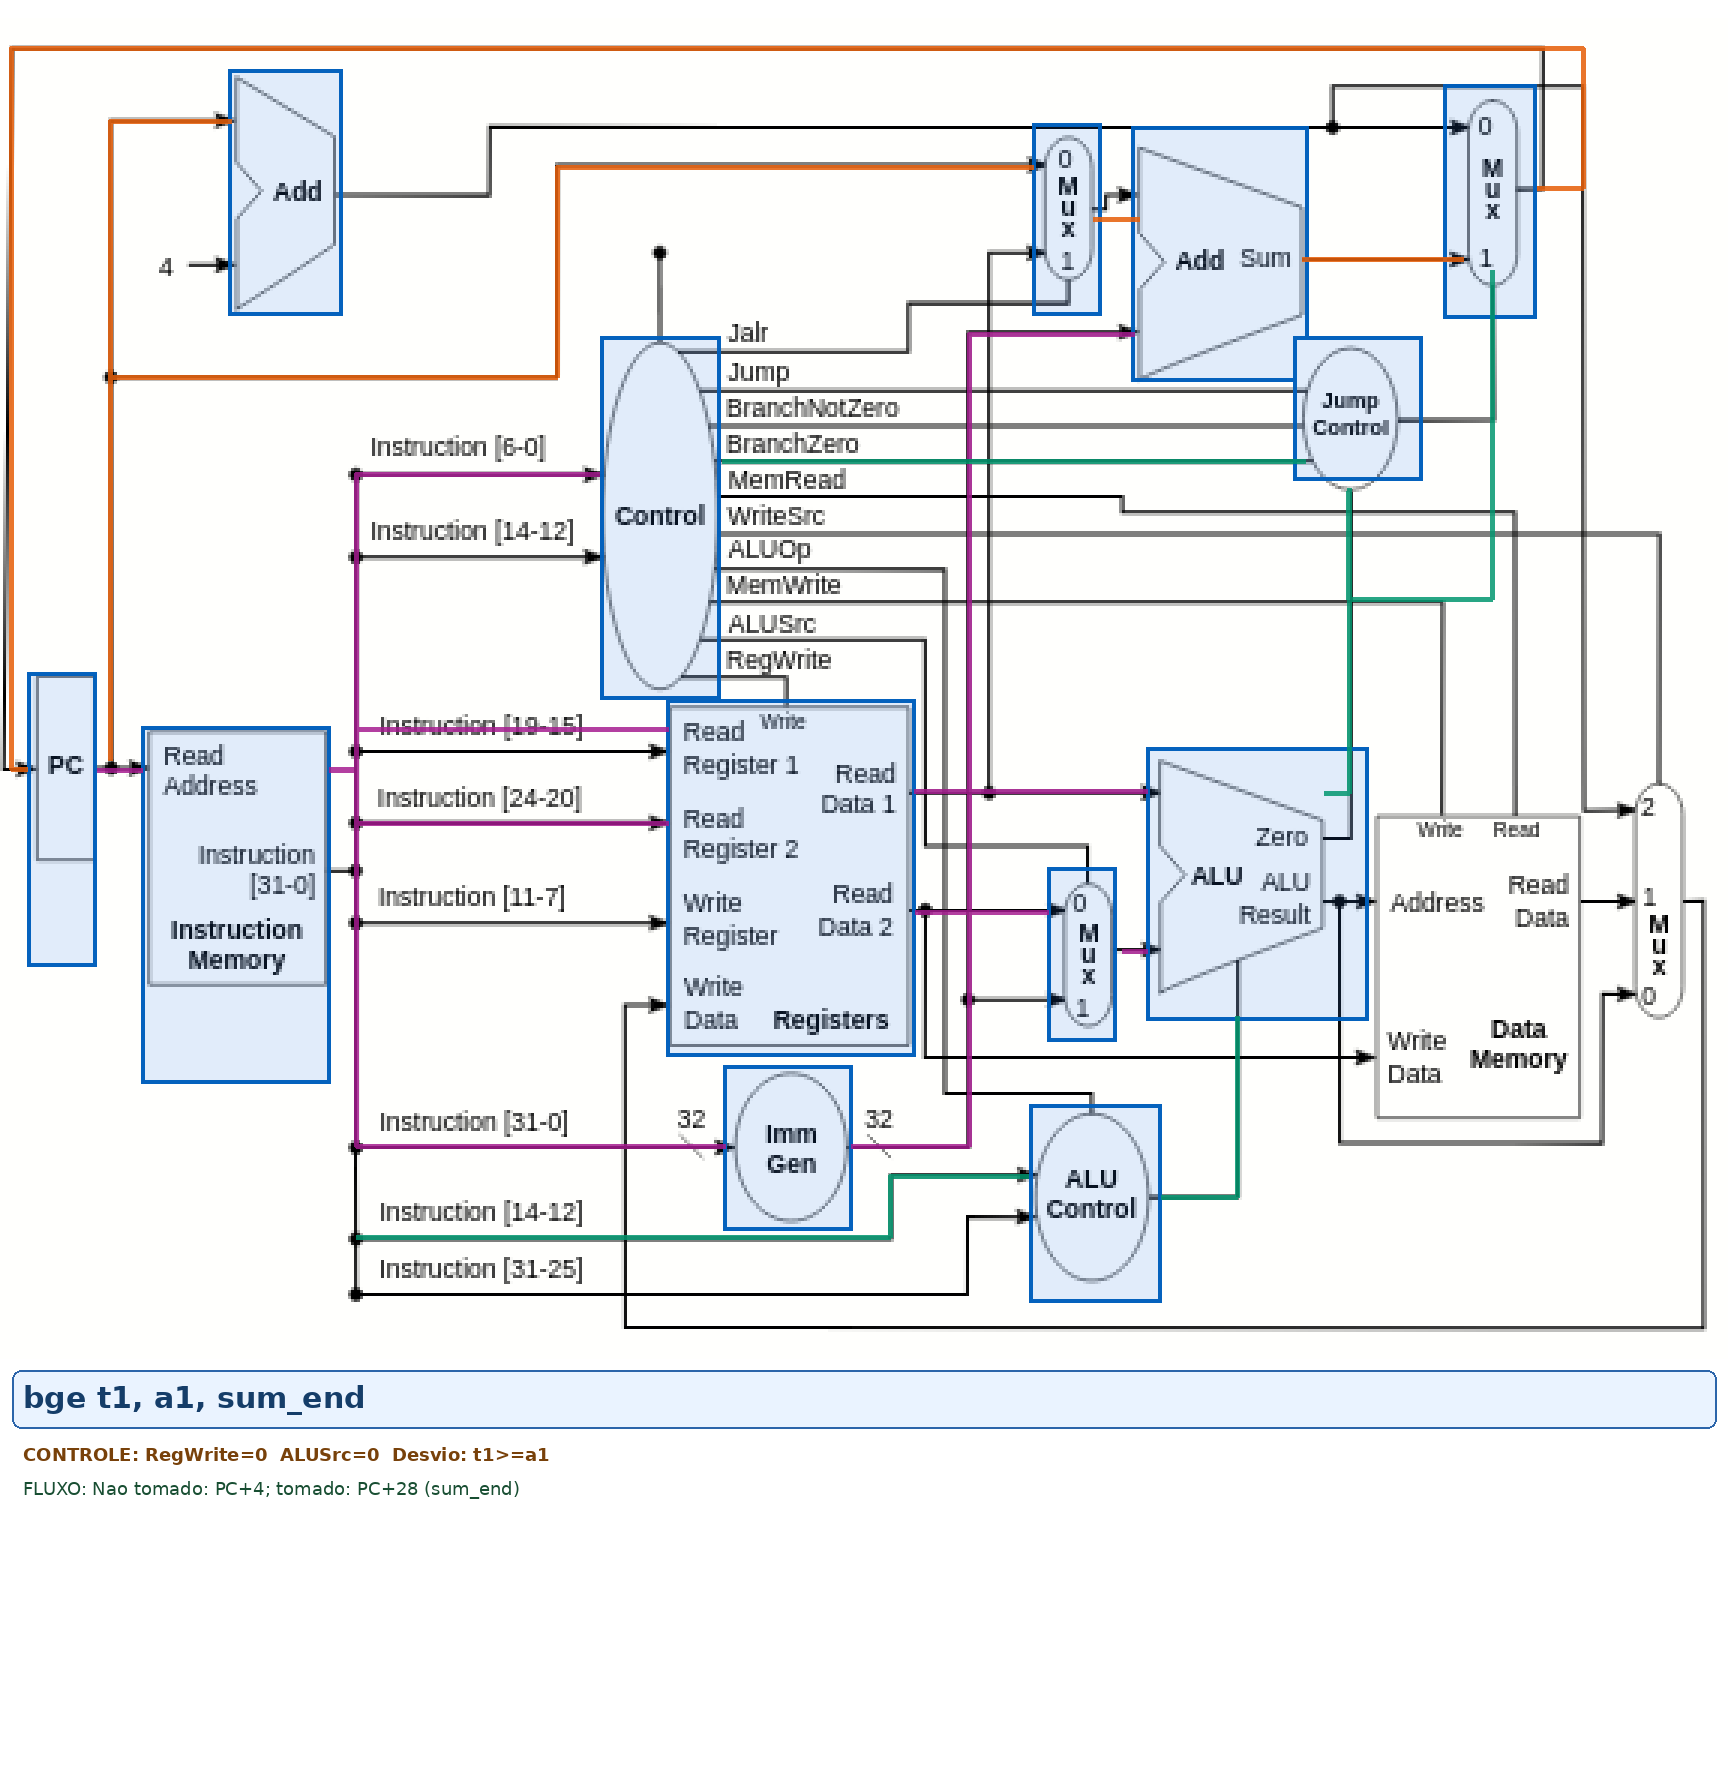
\includegraphics[width=\linewidth]{./img/dp_j/07_datapath.png}
\end{figure}

\clearpage\begin{figure}
    \centering
    \caption*{Jump and Link}
    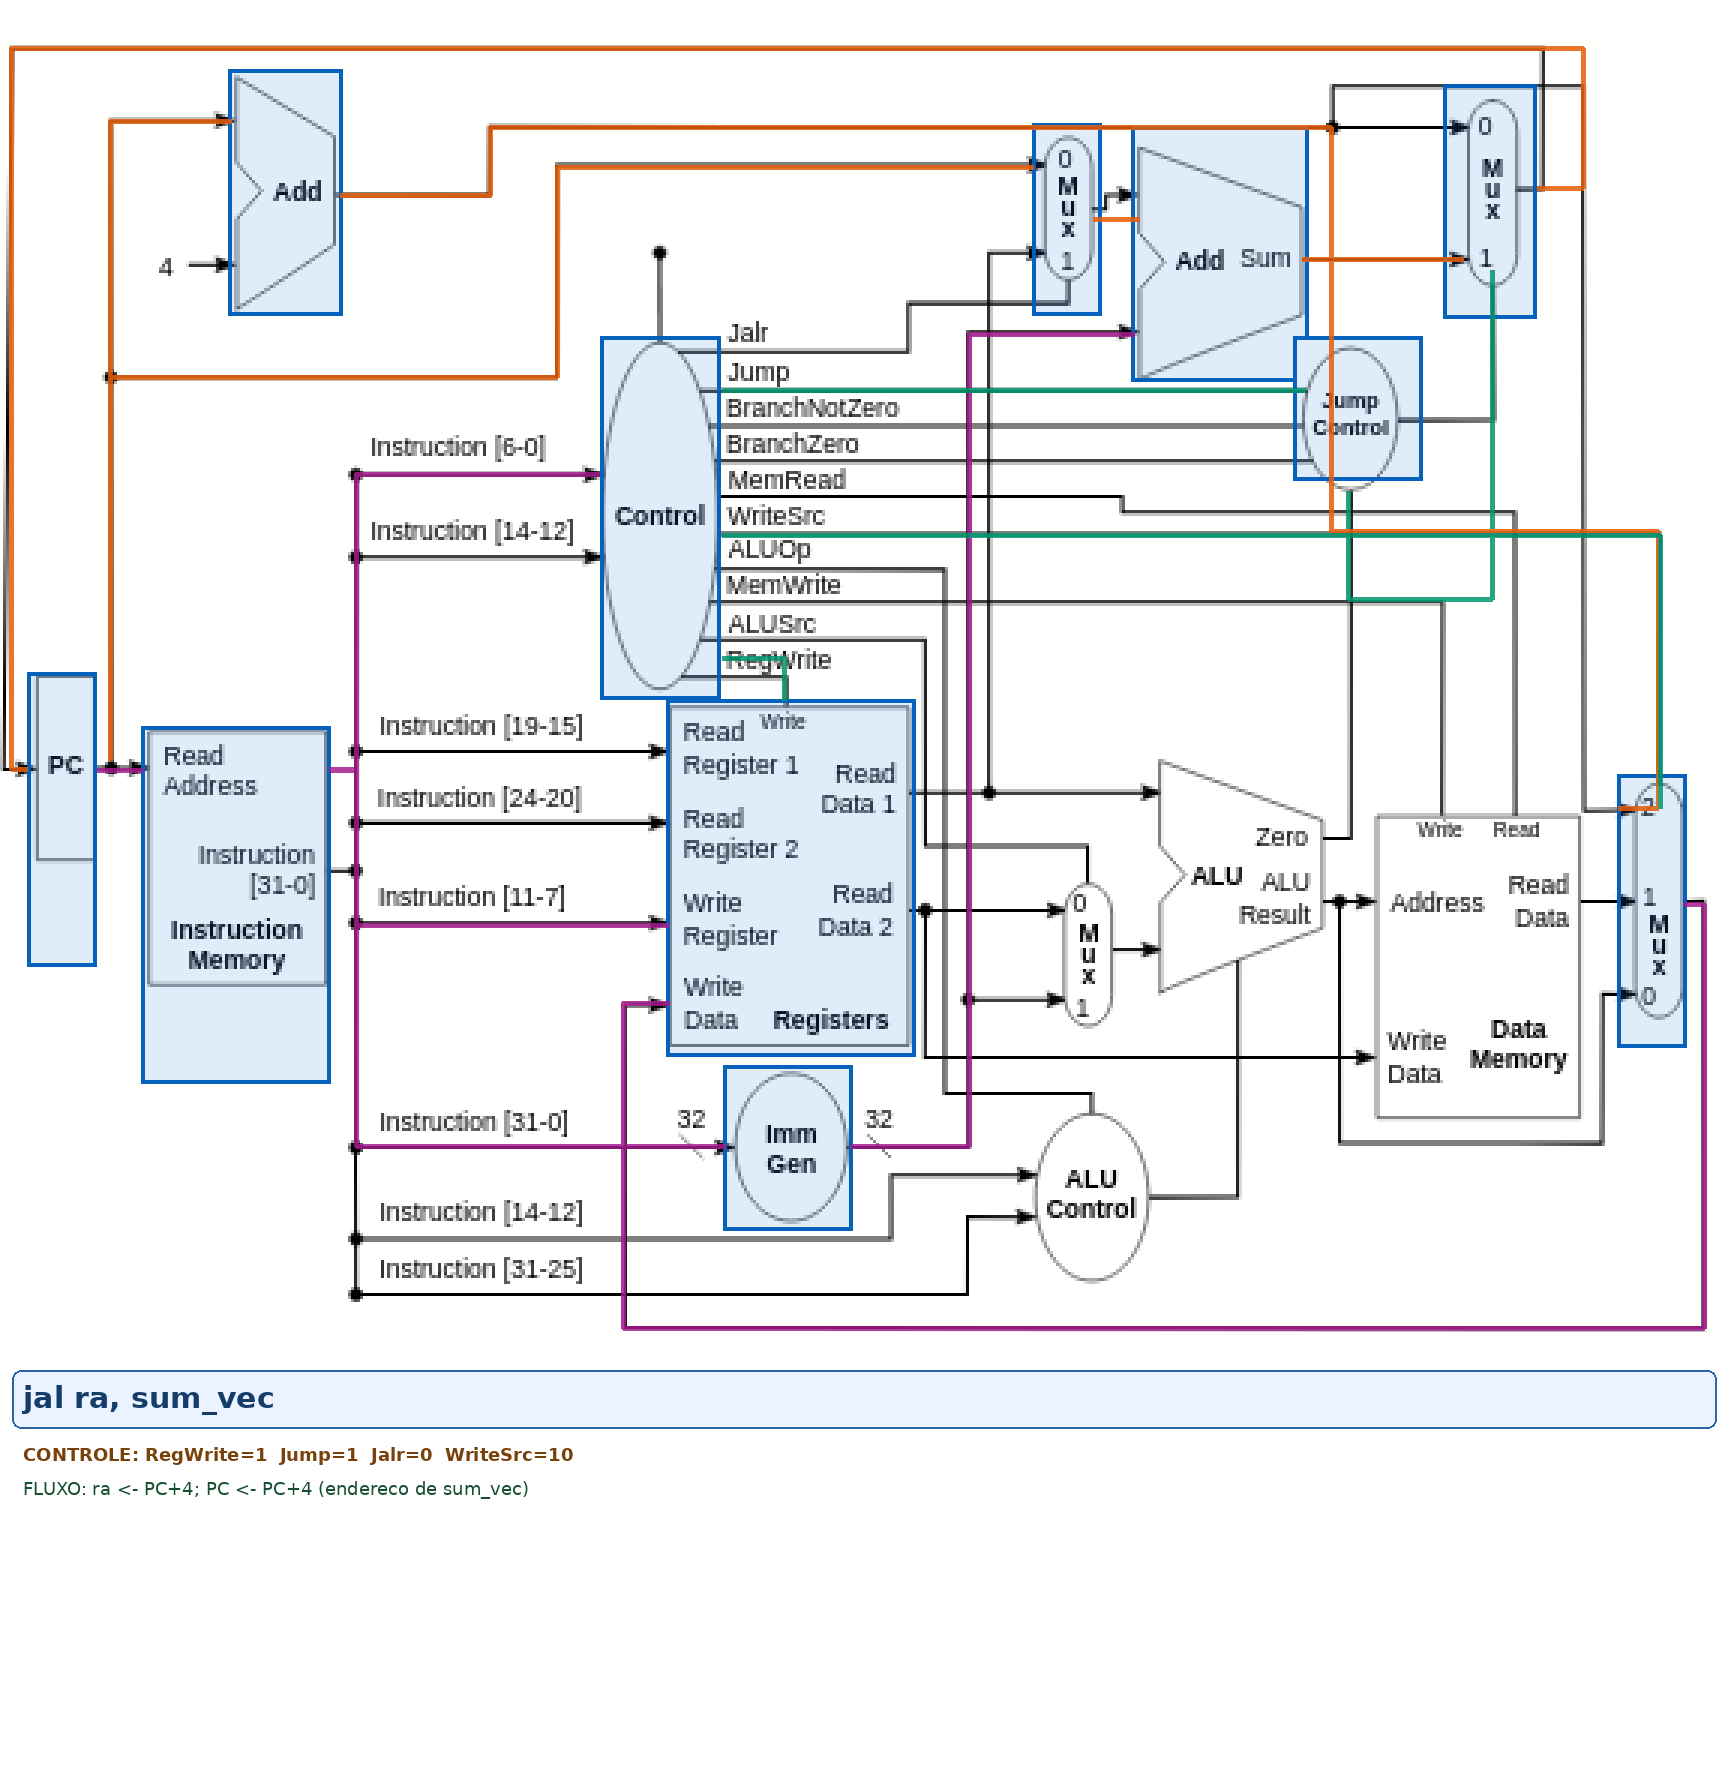
\includegraphics[width=\linewidth]{./img/dp_j/08_datapath.png}
\end{figure}

\clearpage\begin{figure}
    \centering
    \caption*{Jump}
    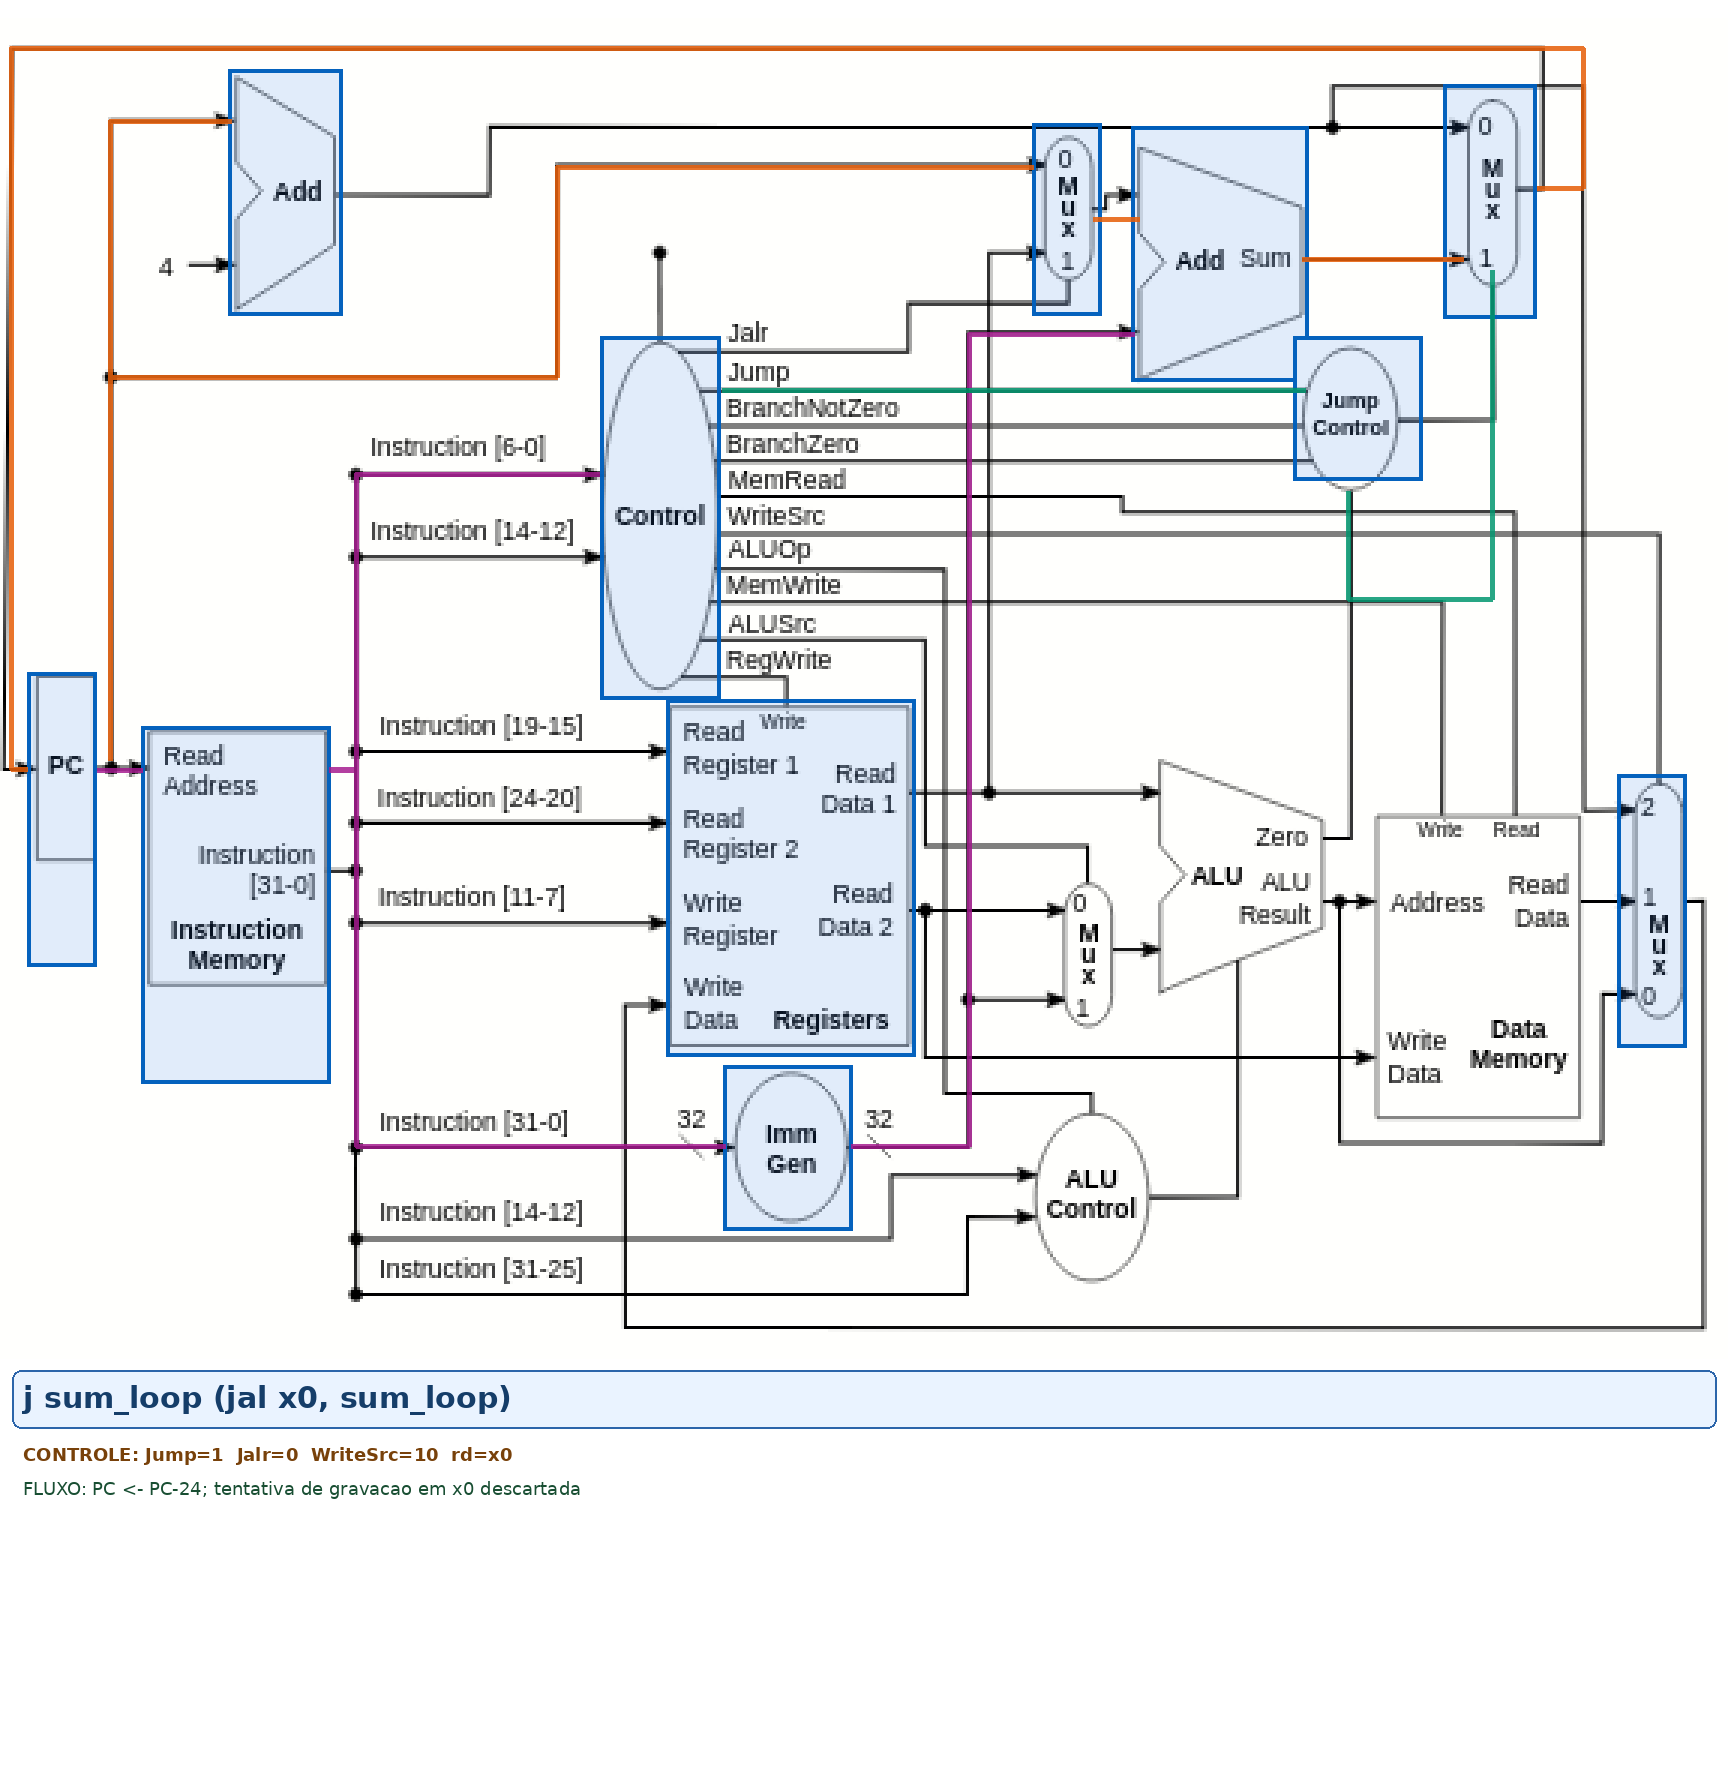
\includegraphics[width=\linewidth]{./img/dp_j/09_datapath.png}
\end{figure}



\section{Parte C}
\begin{figure}[h]
    \hspace*{-3.5cm}
    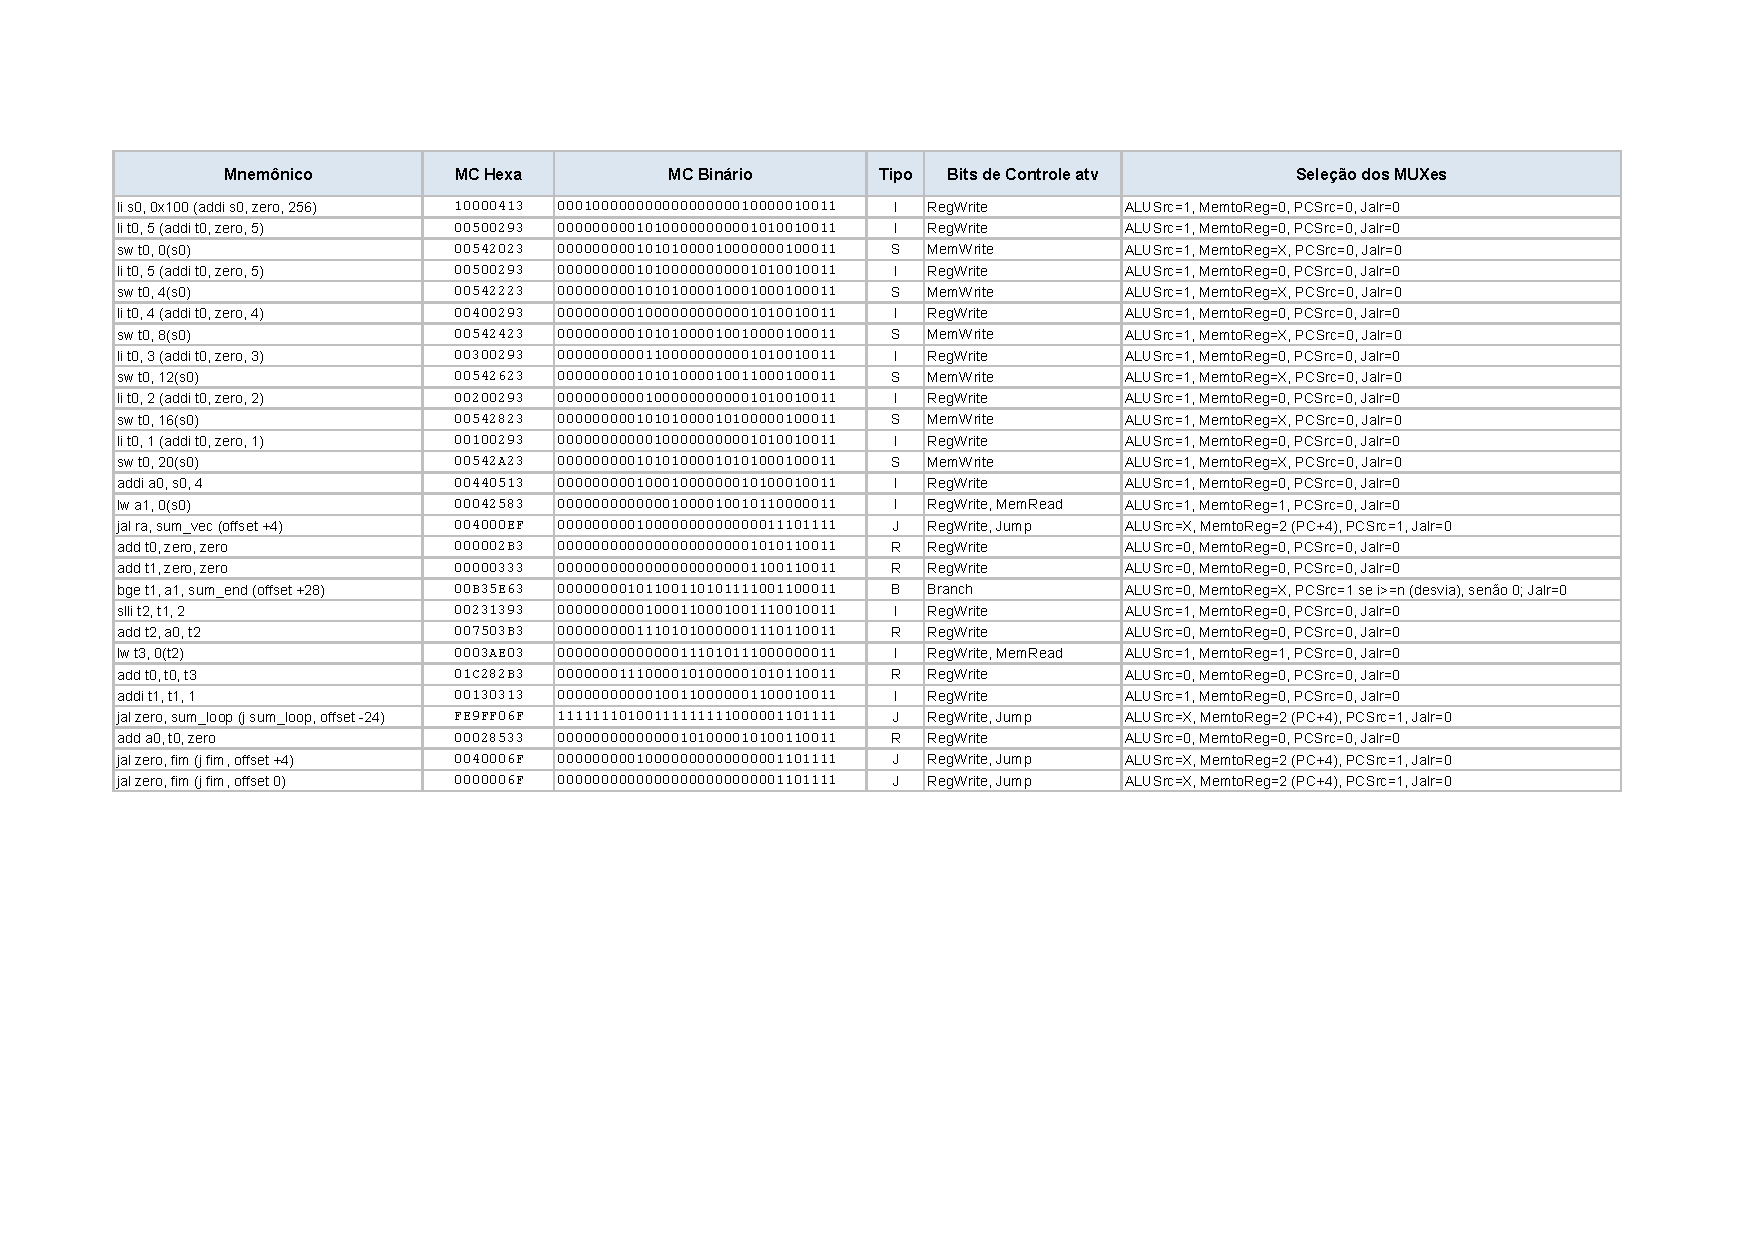
\includegraphics[width=1.5\textwidth,page=1]{./img/tabela-pc.pdf}
\end{figure}

\end{document}
